\documentclass[../../main/main.tex]{subfiles}
\graphicspath{{./figures/}}

\dominitoc
\faketableofcontents

\renewcommand{\mtcSfont}{\small\bfseries}
\renewcommand{\mtcSSfont}{\footnotesize}
\mtcsettitle{minitoc}{}
\mtcsetrules{*}{off}

\makeatletter
\renewcommand{\@chapapp}{Induction -- chapitre}
\makeatother

% \toggletrue{student}
% \toggletrue{corrige}
% \renewcommand{\mycol}{black}
% \renewcommand{\mycol}{gray}

\hfuzz=5.003pt

\begin{document}
\setcounter{chapter}{0}

\settype{book}
\settype{prof}
\settype{stud}

\chapter{Champs magnétiques}
% \epigraph{\openquote\textit{%
% 		Thermodynamics is a funny subject. The first time you go through it, you
% 		don't understand it at all. The second time you go through it, you think you
% 		understand it, except for one or two small points. The third time you go
% 		through it, you know you don't understand it, but by that time you are so
% 		used to it, it doesn't bother you anymore.
% 	}%
% 	\closequote}{Arnold \textsc{Sommerfeld}, $\approx$ 1950}

\vspace*{\fill}

\begin{tcn}(appl)<ctc>"somm"'t'{Sommaire}
	\let\item\olditem
	\vspace{-15pt}
	\minitoc
	\vspace{-25pt}
\end{tcn}

\begin{tcn}[sidebyside, fontupper=\small, fontlower=\small](appl)<ctb>"how"'t'{Capacités exigibles}
	\begin{itemize}[label=\rcheck]
		\item Exploiter une représentation graphique d'un champ vectoriel,
		      identifier les zones de champ uniforme, de champ faible et l'emplacement
		      des sources.

		\item Tracer l'allure des cartes de champs magnétiques pour un aimant droit,
		      une spire circulaire et une bobine longue.

		\item Décrire un dispositif permettant de réaliser un champ magnétique quasi
		      uniforme.

		\item Citer des ordres de grandeur de champs magnétiques : au voisinage
		      d'aimants, dans un appareil d'IRM, dans le cas du champ magnétique
		      terrestre.
	\end{itemize}
	\tcblower
	\begin{itemize}[label=\rcheck]
		\item Exploiter les propriétés de symétrie et d'invariance des sources pour
		      prévoir des propriétés du champ créé.

		\item Évaluer l'ordre de grandeur d'un champ magnétique à partir
		      d'expressions fournies.

		\item Définir le moment magnétique associé à une boucle de courant plane.

		\item Associer à un aimant un moment magnétique par analogie avec une boucle
		      de courant.

		\item Citer un ordre de grandeur du moment magnétique associé à un aimant
		      usuel.
	\end{itemize}
\end{tcn}

\vspace*{\fill}

\newpage

\vspace*{\fill}
% {
% \begin{boxes}
\begin{tcn}[sidebyside, fontupper=\small, fontlower=\small](appl)<ctb>"chek"'t'{L'essentiel}
	\begin{tcn}(defi)<ctc>'t'{Définitions}
		\tcblistof[\paragraph*]{defi}{\hspace*{4.8pt}}
	\end{tcn}
	% \begin{tcn}(rapp)<ctc>'t'{Rappels}
	% 	\tcblistof[\paragraph*]{rapp}{\hspace*{4.8pt}}
	% \end{tcn}
	\begin{tcn}(prop)<ctc>'t'{Propriétés}
		\tcblistof[\paragraph*]{prop}{\hspace*{4.8pt}}
		\tcblistof[\paragraph*]{loi}{\hspace*{4.8pt}}
		% \tcblistof[\paragraph*]{theo}{\hspace*{4.8pt}}
	\end{tcn}
	% \begin{tcn}(coro)<ctc>'t'{Corollaires}
	%   \tcblistof[\paragraph*]{coro}{\hspace*{4.8pt}}
	% \end{tcn}
	% \begin{tcn}(demo)<ctc>'t'{Démonstrations}
	% 	\tcblistof[\paragraph*]{demo}{\hspace*{4.8pt}}
	% 	\tcblistof[\paragraph*]{prev}{\hspace*{4.8pt}}
	% \end{tcn}
	% \begin{tcn}(inte)<ctc>'t'{Interprétations}
	% 	\tcblistof[\paragraph*]{inte}{\hspace*{4.8pt}}
	% \end{tcn}
	% \begin{tcn}(impl)<ctc>'t'{Implications}
	% 	\tcblistof[\paragraph*]{impl}{\hspace*{4.8pt}}
	% \end{tcn}
	% \begin{tcn}(tool)<ctc>'t'{Outils}
	% 	\tcblistof[\paragraph*]{tool}{\hspace*{4.8pt}}
	% \end{tcn}
	% \begin{tcn}(nota)<ctc>'t'{Notations}
	%   \tcblistof[\paragraph*]{nota}{\hspace*{4.8pt}}
	% \end{tcn}
	\begin{tcn}(appl)<ctc>'t'{Applications}
		\tcblistof[\paragraph*]{appl}{\hspace*{4.8pt}}
	\end{tcn}
	% \begin{tcn}(rema)<ctc>'t'{Remarques}
	%   \tcblistof[\paragraph*]{rema}{\hspace*{4.8pt}}
	% \end{tcn}
	% \begin{tcn}(exem)<ctc>'t'{Exemples}
	%   \tcblistof[\paragraph*]{exem}{\hspace*{4.8pt}}
	% \end{tcn}
	% \begin{tcn}*(ror)<ctc>"hart"'t'{Points importants}
	%   \tcblistof[\paragraph*]{ror}{\hspace*{4.8pt}}
	% \end{tcn}
	% \begin{tcn}(impo)<ctc>'t'{Erreurs communes}
	%   \tcblistof[\paragraph*]{impo}{\hspace*{4.8pt}}
	% \end{tcn}
	\tcblower
	% \begin{tcn}(defi)<ctc>'t'{Définitions}
	%   \tcblistof[\paragraph*]{defi}{\hspace*{4.8pt}}
	% \end{tcn}
	% \begin{tcn}(rapp)<ctc>'t'{Rappels}
	%   \tcblistof[\paragraph*]{rapp}{\hspace*{4.8pt}}
	% \end{tcn}
	% \begin{tcn}(prop)<ctc>'t'{Propriétés}
	%   \tcblistof[\paragraph*]{prop}{\hspace*{4.8pt}}
	%   \tcblistof[\paragraph*]{loi}{\hspace*{4.8pt}}
	%   \tcblistof[\paragraph*]{theo}{\hspace*{4.8pt}}
	% \end{tcn}
	% \begin{tcn}(coro)<ctc>'t'{Corollaires}
	%   \tcblistof[\paragraph*]{coro}{\hspace*{4.8pt}}
	% \end{tcn}
	% \begin{tcn}(demo)<ctc>'t'{Démonstrations}
	% 	\tcblistof[\paragraph*]{demo}{\hspace*{4.8pt}}
	% 	\tcblistof[\paragraph*]{prev}{\hspace*{4.8pt}}
	% \end{tcn}
	\begin{tcn}(inte)<ctc>'t'{Interprétations}
		\tcblistof[\paragraph*]{inte}{\hspace*{4.8pt}}
	\end{tcn}
	% \begin{tcn}(impl)<ctc>'t'{Implications}
	% 	\tcblistof[\paragraph*]{impl}{\hspace*{4.8pt}}
	% \end{tcn}
	% \begin{tcn}(tool)<ctc>'t'{Outils}
	%   \tcblistof[\paragraph*]{tool}{\hspace*{4.8pt}}
	% \end{tcn}
	% \begin{tcn}(nota)<ctc>'t'{Notations}
	%   \tcblistof[\paragraph*]{nota}{\hspace*{4.8pt}}
	% \end{tcn}
	\begin{tcn}(odgr)<ctc>'t'{Ordres de grandeur}
		\tcblistof[\paragraph*]{odgr}{\hspace*{4.8pt}}
	\end{tcn}
	% \begin{tcn}(appl)<ctc>'t'{Applications}
	% 	\tcblistof[\paragraph*]{appl}{\hspace*{4.8pt}}
	% \end{tcn}
	% \begin{tcn}(rema)<ctc>'t'{Remarques}
	%   \tcblistof[\paragraph*]{rema}{\hspace*{4.8pt}}
	% \end{tcn}
	% \begin{tcn}(exem)<ctc>'t'{Exemples}
	% 	\tcblistof[\paragraph*]{exem}{\hspace*{4.8pt}}
	% \end{tcn}
	\begin{tcn}*(ror)<ctc>"hart"'t'{Points importants}
		\tcblistof[\paragraph*]{ror}{\hspace*{4.8pt}}
	\end{tcn}
	\begin{tcn}(impo)<ctc>'t'{Erreurs communes}
		\tcblistof[\paragraph*]{impo}{\hspace*{4.8pt}}
	\end{tcn}
\end{tcn}
% \end{boxes}
% }%

\vspace*{\fill}
\newpage

\section{Introduction}
\subsection{Notion de champ en physique}
La notion de champ est omniprésente en physique.
\begin{tcb}(defi){Champ}
	Un \textbf{champ} est une grandeur physique définie en tout point M. Sa
	valeur dépend en général également du temps. Il peut être~:
	\begin{itemize}
		\setlength{\fboxsep}{3mm}
		\item[b]{Scalaire}: la grandeur est un scalaire (température,
		pression…). On l'écrit $\boxed{\psw{X (\Mr,t)}}$~;
		\item[b]{Vectoriel}: la grandeur physique est un vecteur (force,
		vitesse…). On l'écrit $\boxed{\psw{\vv{X}(\Mr,t)}}$~;
		\item[b]{Stationnaire}: la grandeur physique ne \textbf{dépend pas du
			temps}~: $\boxed{\psw{X (\Mr,\dcancel{t}) = X(\Mr)}}$~;
		\item[b]{Uniforme}: la grandeur ne \textbf{dépend pas de la position}~:
		$\boxed{\psw{X (\dcancel{\Mr},t) = X(t)}}$.
	\end{itemize}
	% \begin{itemize}
	% 	\item Lorsque la grandeur physique est un scalaire (température,
	% 	      pression…), on parle de \textbf{champ scalaire}~: \psw{$X (\Mr,t)$~;}
	% 	\item Lorsqu'elle est un vecteur (force, vitesse…), on parle de
	% 	      \textbf{champ vectoriel}~: \psw{$\vv{X}(\Mr,t)$~;}
	% 	\item Lorsqu'elle ne dépend pas du temps, le champ est
	% 	      \textbf{stationnaire}~: $X (\Mr,\dcancel{t}) = X(\Mr)$~;
	% 	\item Lorsque la valeur ne dépend pas de la position dans l'espace, le
	% 	      champ est \textbf{uniforme}~: $X (\dcancel{\Mr},t) = X (t)$.
	% \end{itemize}
\end{tcb}
\begin{tcb}(exem)<lftt>'l'{Champs scalaire et vectoriel}
	\begin{itemize}
		\item
		      \psw{%
			      À deux dimensions, le champ d'\textbf{altitude} peut être défini sur une
			      carte de randonnée. En tout point $(x,y)$ de la carte, une grandeur
			      \textbf{scalaire} $z(x,y)$ est définie.
		      }%

		\item
		      \psw{%
			      On peut définir des champs \textbf{scalaires} de \textbf{pression} $p
				      (x,y)$ ou de \textbf{température} $T (x,y)$ sur une carte
			      météorologique.
		      }%
		\item
		      \psw{%
			      On peut définir un champ de \textbf{vitesse} du vent $\vv{v}(x,y)$ où un
			      \textbf{vecteur} est défini en tout point d'une carte~: sa
			      \textbf{direction} autant que sa \textbf{norme} importent~;
		      }%
		\item
		      \psw{%
			      On peut aussi définir un champ de \textbf{force gravitationnelle} $\Ff
				      (x,y,z)$ dans tout l'espace, qui pointe toujours vers le centre de la
			      Terre.
		      }%
	\end{itemize}
	\noindent
	\begin{minipage}[t]{.5\linewidth}
		\centering
		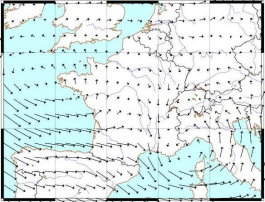
\includegraphics[scale=1]{champ_vent}
		\captionof{figure}{Champ vectoriel du vent.}
		\label{fig:chpvent}
	\end{minipage}
	\hfill
	\begin{minipage}[t]{.5\linewidth}
		\centering
		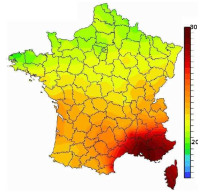
\includegraphics[scale=1]{champ_T}
		\captionof{figure}{Champ scalaire de la température.}
		\label{fig:chpT}
	\end{minipage}
\end{tcb}

\begin{tcb*}[sidebyside, righthand ratio=.3](defi){Cartes et lignes de champ}
	Pour représenter un champ vectoriel, on utilise des~:
	\begin{itemize}
		\item[b]{cartes de champ}: à chaque point de l'espace est associé un
		\textbf{vecteur} donnant le \textbf{sens et la norme} du champ~;

		\item[b]{lignes de champ}: ce sont les \textbf{courbes orientées},
		\textbf{tangentes au champ} que l'on
		obtient en suivant le champ de proche en proche. Chaque ligne indique le
		\textbf{sens} du champ.
	\end{itemize}
	% \psw{
	% 	Les \textbf{lignes de champ} sont des courbes \textbf{orientées} tangentes
	% 	en tout point au champ magnétique. Elles donnent la direction \textbf{et le
	% 		sens} du champ magnétique en tout point.
	% }
	\tcblower
	\begin{center}
		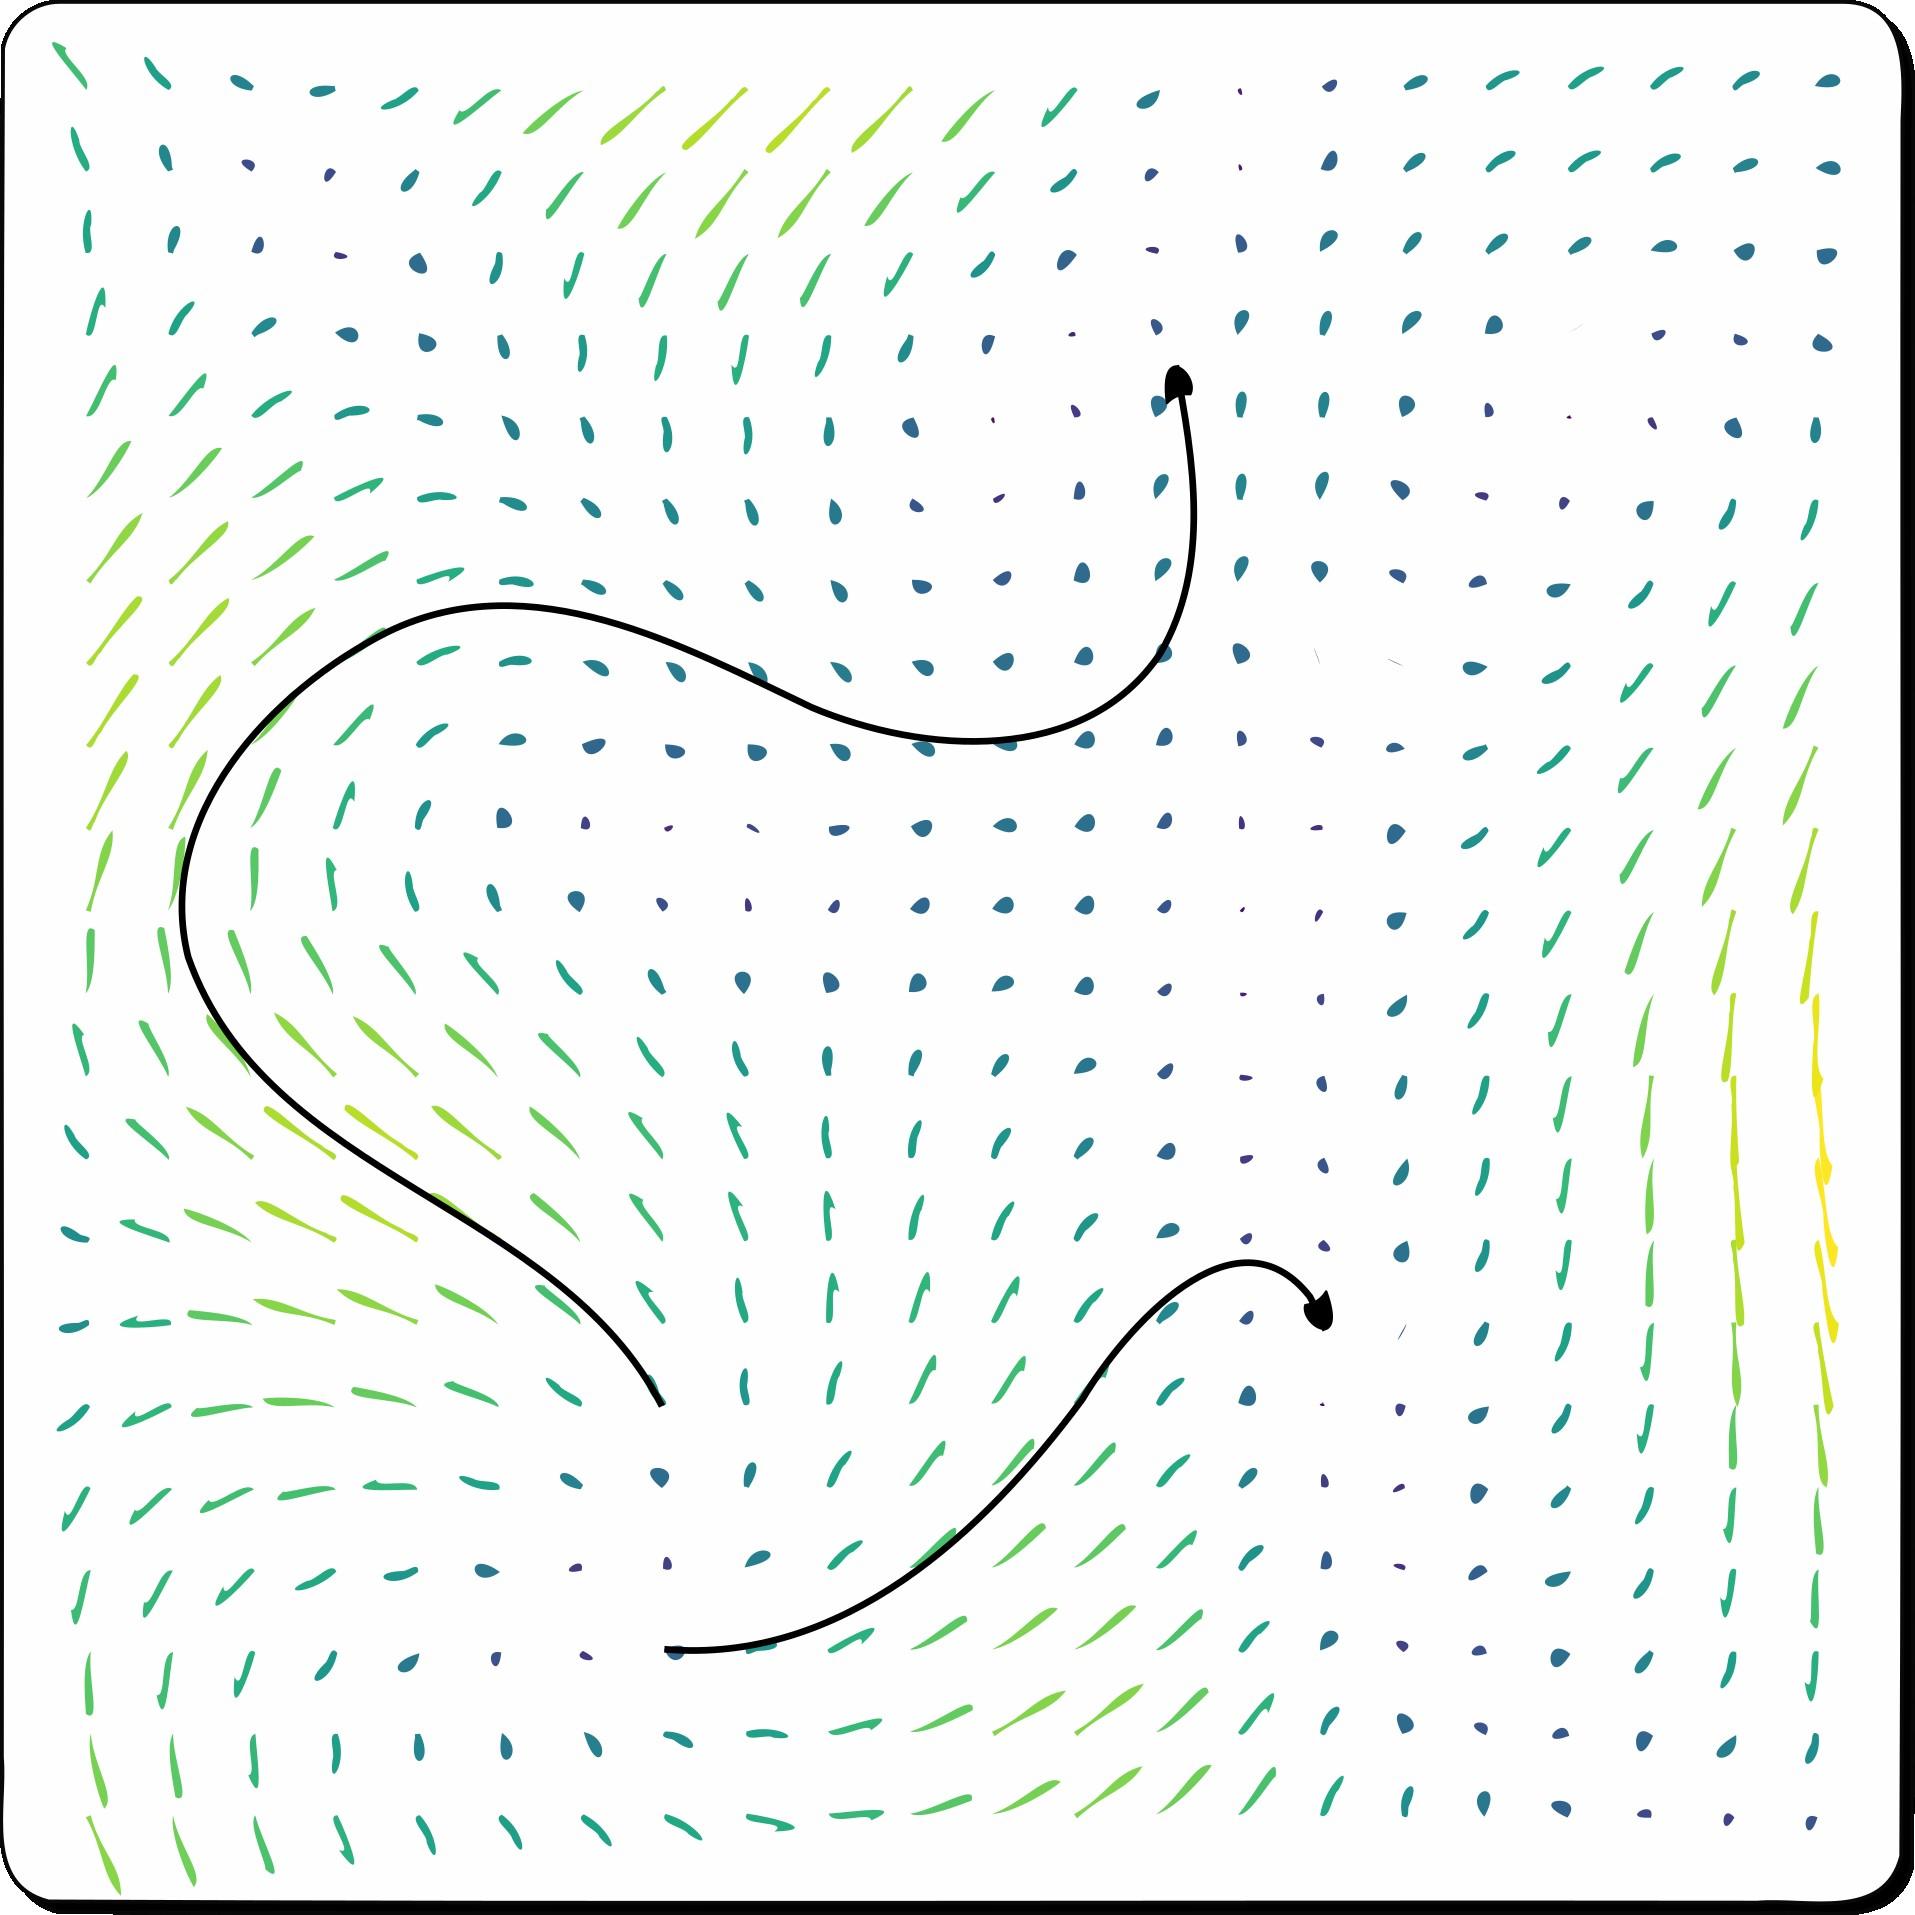
\includegraphics[width=\linewidth]{ldc_qlcq}
	\end{center}
\end{tcb*}

\subsection{Interaction entre aimants}
\textbf{Observations expérimentales}

\begin{table}[htbp!]
	\centering
	\caption{Interactions entre aimants}
	\begin{tabularx}{\linewidth}{YYY}
		\toprule
		\textbf{Situation A}
		 &
		\textbf{Situation B}
		 &
		\textbf{Situation C}
		\\
		\midrule
		\begin{center}
			\sswitch{
				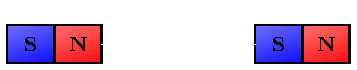
\includegraphics[width=\linewidth]{inter_aimant_SN-SN_stud}
			}{
				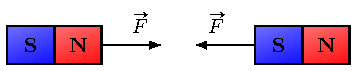
\includegraphics[width=\linewidth]{inter_aimant_SN-SN}
			}
		\end{center}
		 &
		\begin{center}
			\sswitch{
				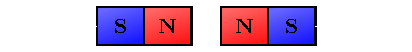
\includegraphics[width=\linewidth]{inter_aimant_SN-NS_stud}
			}{
				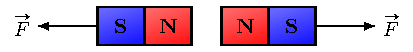
\includegraphics[width=\linewidth]{inter_aimant_SN-NS}
			}
		\end{center}
		 &
		\begin{center}
			\sswitch{
				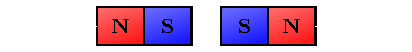
\includegraphics[width=\linewidth]{inter_aimant_NS-SN_stud}
			}{
				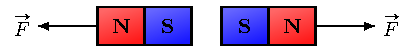
\includegraphics[width=\linewidth]{inter_aimant_NS-SN}
			}
		\end{center}
		\\
		\bottomrule
	\end{tabularx}
\end{table}

\begin{itemize}
	\item Deux aimants peuvent s'\textbf{attirer ou se repousser} selon la façon
	      dont on les oriente~;
	\item ~
	      \smallbreak
	      \vspace{-30pt}
	      \noindent
	      \begin{minipage}[c]{.80\linewidth}
		      Le champ magnétique peut être mis en évidence avec un petit aimant en
		      forme d'aiguille (boussole)~;
	      \end{minipage}
	      \begin{minipage}[c]{.19\linewidth}
		      \begin{center}
			      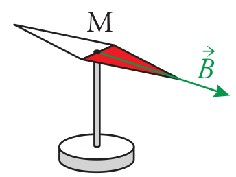
\includegraphics[width=.7\linewidth]{boussole}
		      \end{center}
	      \end{minipage}
\end{itemize}

\begin{tcb*}[sidebyside, righthand ratio=.2](defi){Boussole}
	Une boussole est une aiguille aimantée libre de tourner. On appelle
	\textbf{nord magnétique} l'extrémité qui pointe vers le \textbf{nord
		géographique}.
	\tcblower
	\begin{center}
		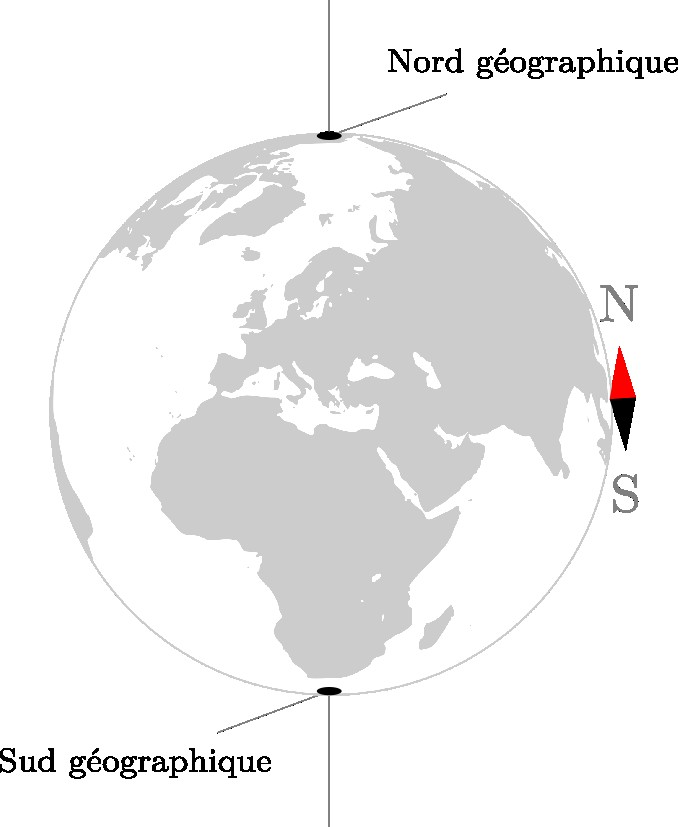
\includegraphics[width=\linewidth]{bouss_terre.jpg}
	\end{center}
\end{tcb*}
% Pour quantifier ces effets, on va introduire la notion de champ magnétique.

\subsection{Le vecteur champ magnétique}
% La direction de l'aiguille aimantée en un point indique la direction du champ
% magnétique.
\begin{tcb*}(defi){Champ magnétique}
	Le \textbf{champ magnétique} est caractérisé par un
	\textbf{vecteur}, noté $\Bf (\Mr,t)$, défini par~:
	\begin{itemize}
		\item[b]{sa direction}: \psw{celle d'une aiguille aimantée~;}
		\item[b]{son sens}: \psw{va du pôle Sud au pôle Nord de l'aiguille~;}
		\item[b]{sa norme}: \psw{s'exprime en tesla (\si{T}).}
	\end{itemize}
\end{tcb*}

\section{Sources et cartes de champ magnétique}
\subsection{Aimant droit}
\label{ssec:aimdroit}
\noindent
\begin{minipage}[c]{.48\linewidth}
	Pour visualiser un champ magnétique d'un aimant, on peut utiliser de la limaille
	de fer. Les grains de limaille, de formes allongées, se transforment en petits
	aimants sous l'action du champ magnétique~; ils se comportent ainsi comme de
	petits boussoles qui s'orientent parallèlement au champ magnétique. On constate
	que les grains de limaille forment des courbes particulières allant d'un pôle de
	l'aimant vers l'autre, voir Figure~\ref{fig:lim1}.
\end{minipage}
\hfill
\begin{minipage}[c]{.48\linewidth}
	\begin{center}
		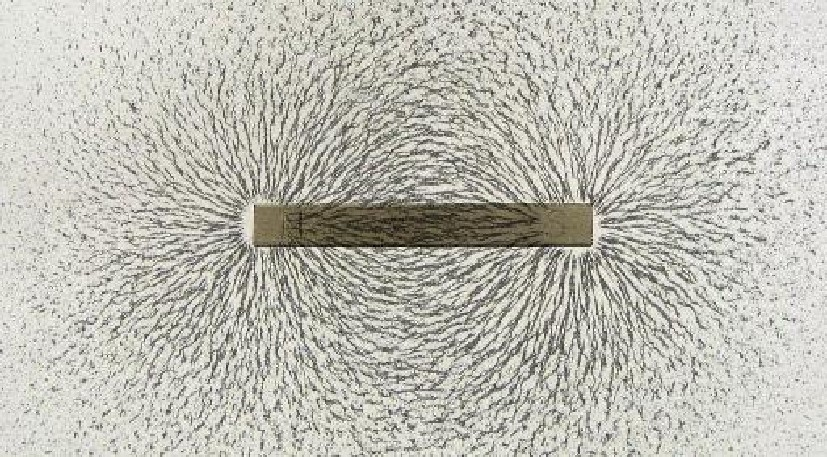
\includegraphics[scale=1]{aimdroit_lim.jpg}
		\captionof{figure}{Observation du champ magnétique d'un aimant au travers de
			son action sur l'orientation de grains de limaille de fer.}
		\label{fig:lim1}
	\end{center}
\end{minipage}
% \begin{figure}[h]
% 	\centering
% 	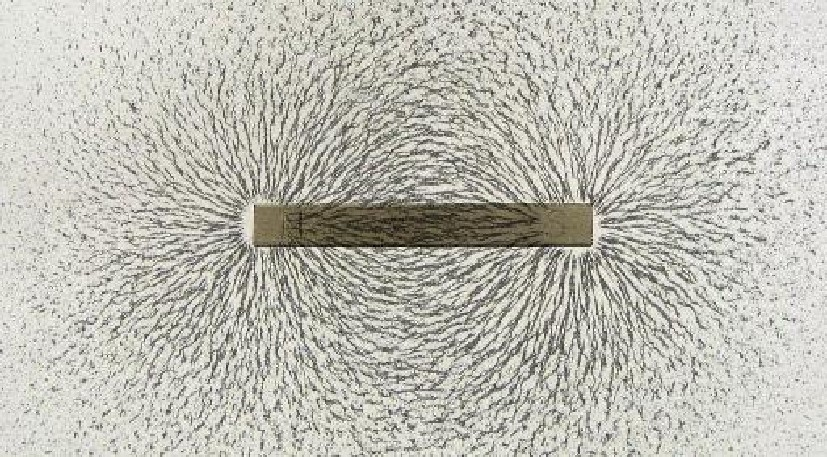
\includegraphics[scale=1]{aimdroit_lim.jpg}
% 	\caption{Observation du champ magnétique d'un aimant au travers de son action
% 		sur l'orientation de grains de limaille de fer.}
% 	\label{fig:lim1}
% \end{figure}

On en tire l'observation suivante~:
\begin{tcb*}(prop){Géométrie des lignes de champ}
	\psw{
		Les lignes de champ du champ magnétique sont des \textbf{courbes fermées}
		qui sortent de l'aimant par le pôle Nord et y rentrent par le pôle Sud.
	}
\end{tcb*}
Schématiquement, on les représente de la manière suivante~:

\begin{figure}[h]
	\centering
	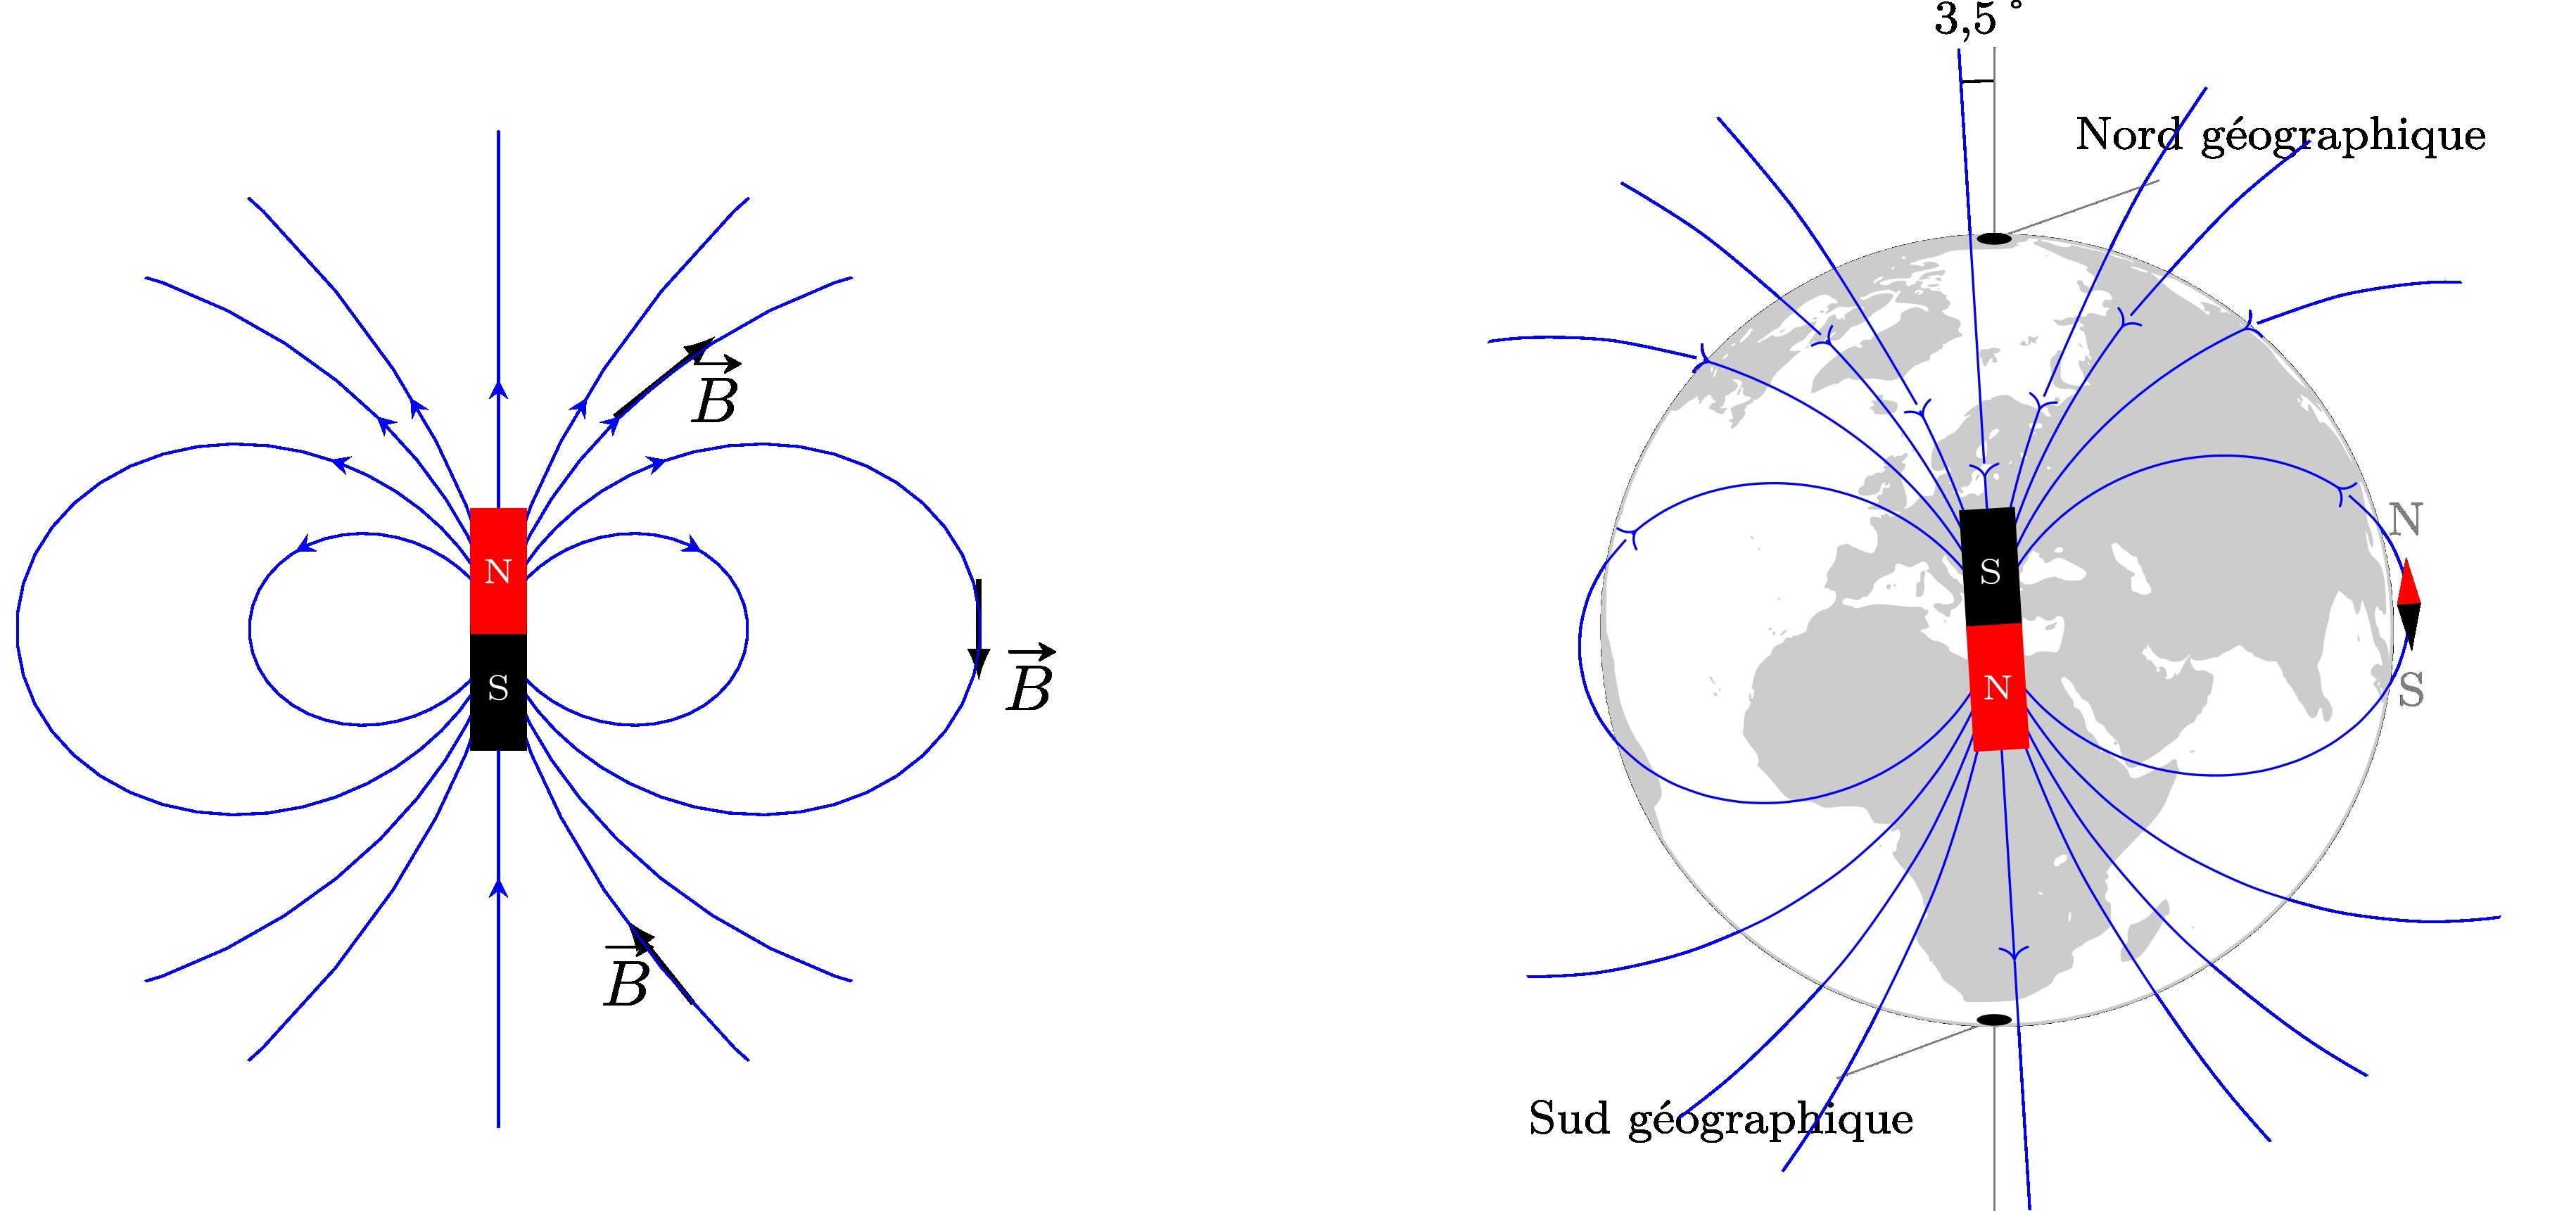
\includegraphics[scale=1]{aimdroit.jpg}
	\caption{Schématisation des lignes de champ dans un aimant droit, et
		schématisation du champ magnétique de la Terre comme celui d'un aimant droit.
		Une boussole à la surface de la Terre s'aligne sur le \textbf{pôle Sud magnétique}
		de la Terre, qui est proche du Nord géographique.}
	\label{fig:aimdroitterre}
\end{figure}

La Terre se comporte alors comme un gigantesque aimant. Son Sud magnétique se
situe au nord géographique, de sorte à ce que les nords magnétiques des
boussoles s'orientent vers le nord géographique.

\subsection{Champs magnétiques créés par des courants}
\label{ssec:chpcour}

En 1820, \textsc{Œrsted} découvre qu'un \textbf{fil parcouru par un courant
	dévie une aiguille aimantée}~: c'est la première preuve historique qu'un courant
électrique créé un champ magnétique. De plus, en changeant le sens du courant,
on change le sens de l'aiguille. Regardons différentes manières de réaliser
cette expérience~:

\subsubsection{Bobine plate}
\label{sssec:bplate}
Une bobine plate est un fil électrique de forme circulaire. On refait une
expérience avec de la limaille de fer~: on retrouve alors des lignes qui sont
analogues à celles créées par l'aimant, si on le plaçait perpendiculairement à
la spire (ici, vertical).

\begin{figure}[h]
	\noindent
	\begin{minipage}[c]{.48\linewidth}
		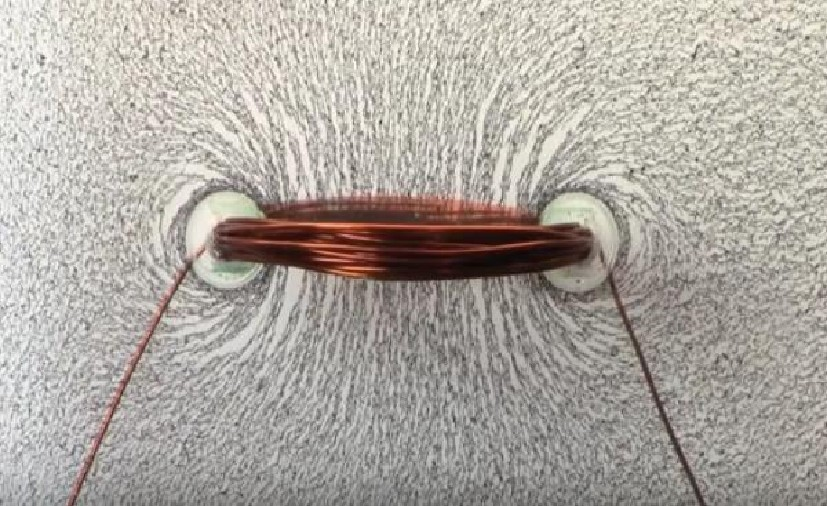
\includegraphics[width=\linewidth]{bplate_lim.jpg}
	\end{minipage}
	\hfill
	\begin{minipage}[c]{.48\linewidth}
		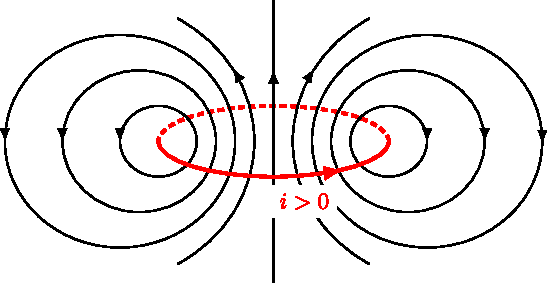
\includegraphics[width=\linewidth]{bplate_chp}
	\end{minipage}
	% 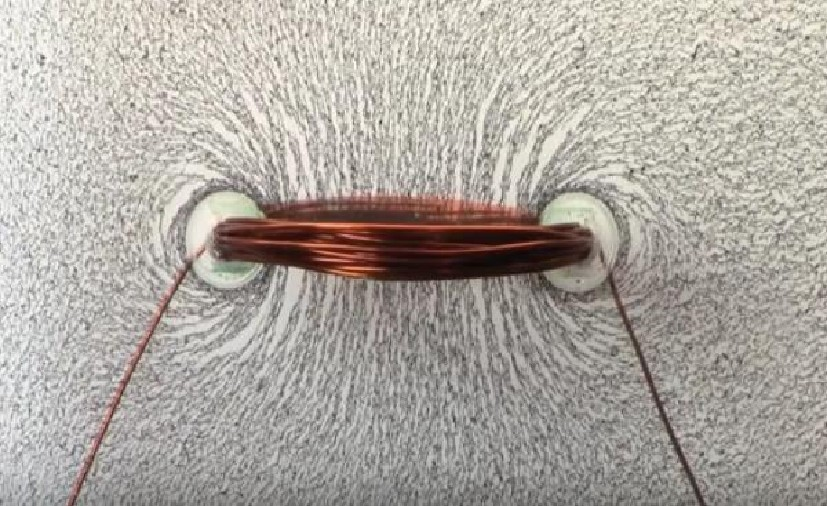
\includegraphics[width=.48\linewidth]{bplate_lim.jpg}
	% 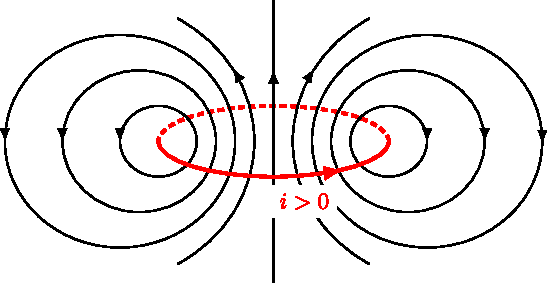
\includegraphics[width=.48\linewidth]{bplate_chp.pdf}
	\caption{Observation du champ créé par une bobine plate~: limaille de fer et
		schématisation.}
	\label{fig:bplate}
\end{figure}
On observe alors la similitude suivante~:
\begin{tcb*}(prop){Comparaison LdC aimant/bobine}
	\begin{center}
		\psw{%
			Les lignes de champ d'une \textbf{bobine plate} s'apparentent à celles
			d'un \textbf{aimant droit}.
		}%
	\end{center}
\end{tcb*}

\subsubsection{Solénoïde}
\label{sssec:solen}
\begin{tcb*}(defi){Solénoïde}
	\begin{center}
		\psw{
			En enroulant un fil le long d'un cylindre, on fabrique un
			\textbf{solénoïde}, ou bobine longue.
		}
	\end{center}
\end{tcb*}

\begin{figure}[h]
	\noindent
	\begin{minipage}[c]{.20\linewidth}
		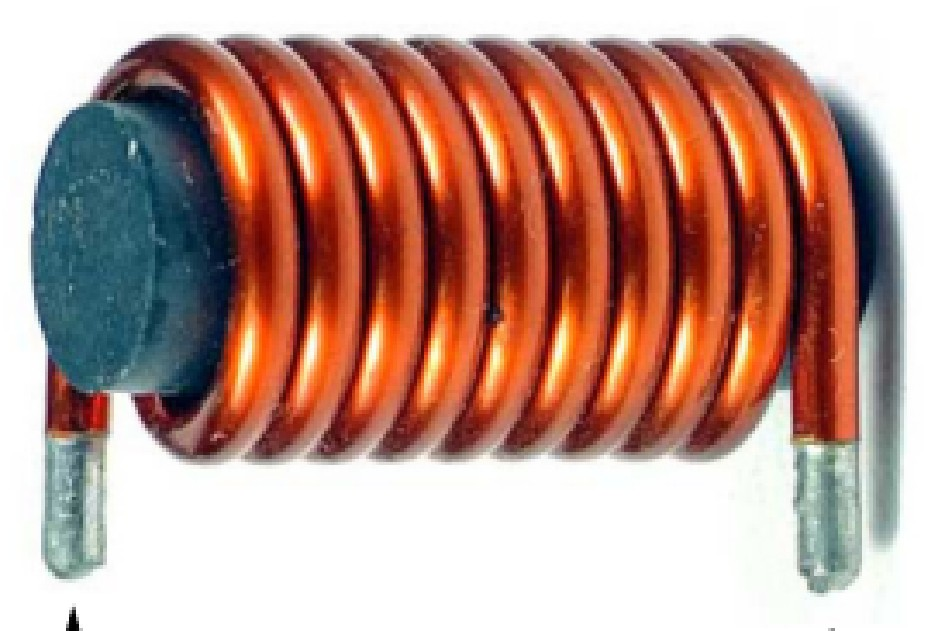
\includegraphics[scale=1]{sol_phot.jpg}
	\end{minipage}
	\hfill
	\begin{minipage}[c]{.70\linewidth}
		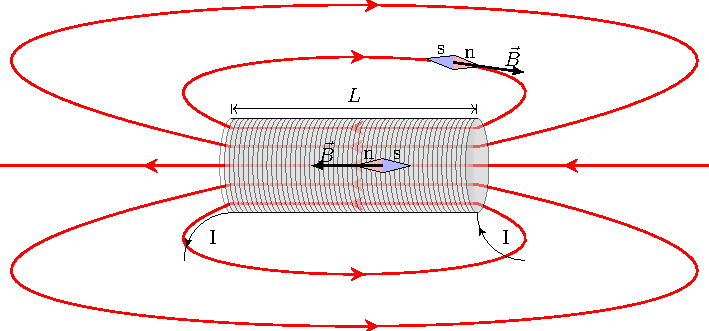
\includegraphics[width=\linewidth]{sol_chp}
	\end{minipage}
	% 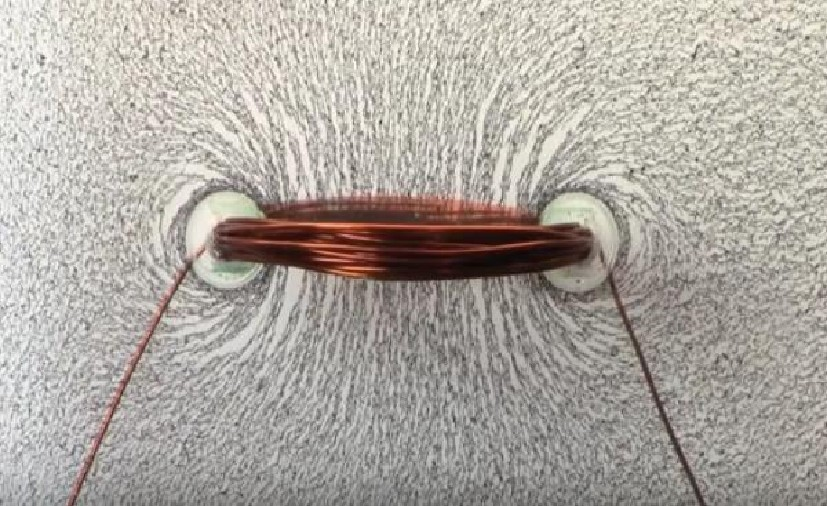
\includegraphics[width=.48\linewidth]{bplate_lim.jpg}
	% 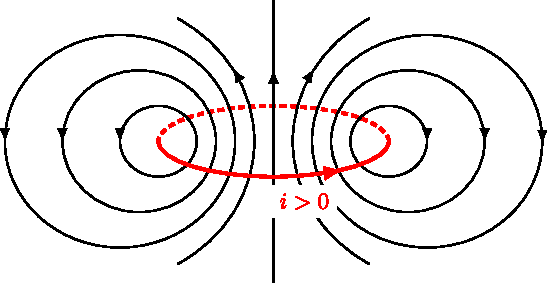
\includegraphics[width=.48\linewidth]{bplate_chp.pdf}
	\caption{Photo et représentation d'un solénoïde avec lignes de champ.}
	\label{fig:sol1}
\end{figure}

% \noindent
% \begin{minipage}[c]{.5\linewidth}
% 	\centering
% 	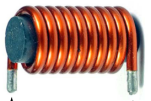
\includegraphics[scale=1]{sol_phot}
% 	\captionof{figure}{Photo d'un solénoïde.}
% 	\label{fig:solphot}
% \end{minipage}
% \hfill
% \begin{minipage}[c]{.5\linewidth}
% 	\centering
% 	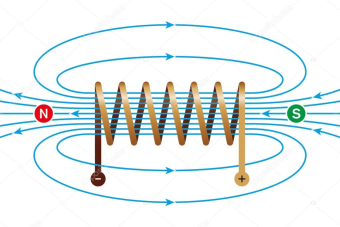
\includegraphics[width=\linewidth]{sol1}
% 	\captionof{figure}{Représentation d'un solénoïde avec lignes de champ.}
% 	\label{fig:sol1}
% \end{minipage}

Étendre une bobine a pour effet de rendre les lignes de champ parallèles dans le
solénoïde. En dehors, les \textbf{lignes de champ} se referment de façon
\textbf{analogue} encore une fois à celle de l'\textbf{aimant droit}.

\section{Intensité du champ magnétique}
\label{sec:intchp}
\paragraph*{Expérience} Plus la boussole est proche de l'aimant, plus elle
s'aligne \textbf{rapidement} sur le champ magnétique. C'est au travers de ses
effets sur les courants, les aimants etc. que nous mesurons l'intensité du champ
magnétique, exprimé en tesla (\si{T}).
\begin{tcb*}(odgr)<lftt>'l'{Intensité du champ magnétique}
	\begin{center}
		\begin{tabular}{lcccc}
			\toprule
			\textbf{Source}
			 &
			Terre
			 &
			Aimant
			 &
			Électroaimant
			 &
			IRM
			\\
			\textbf{Norme}
			 &
			$ \approx \SI{5e-5}{T} $
			 &
			$ \approx \SIrange{0.01}{0.5}{T} $
			 &
			$ \approx \SIrange{1}{10}{T} $
			 &
			$ \approx \SI{10}{T} $
			\\
			\bottomrule
		\end{tabular}
	\end{center}
	% \begin{itemize}
	% 	\item champ créé par un aimant        $ \approx \SIrange{0.01}{0.5}{T} $~;
	% 	\item champ créé par un électroaimant $ \approx \SIrange{1}{10}{T} $~;
	% 	\item champ créé par un IRM           $ \approx \SI{10}{T} $~;
	% \end{itemize}
\end{tcb*}

\subsection{Lire une intensité sur une carte}
\paragraph*{Observation}
En reprenant l'exemple précédent du solénoïde, on remarque qu'une aiguille
s'alignera \textbf{rapidement} si elle est \textbf{proche du solénoïde}, voire à
l'intérieur, mais de plus en plus lentement quand on s'en éloigne. On a donc les
deux observations suivantes en \textbf{augmentant la distance} à la bobine~:
\begin{itemize}
	\item \psw{les lignes de champ s'\textbf{écartent} les unes des autres~;}
	\item \psw{l'intensité du champ \textbf{décroît}.}
\end{itemize}
Ces deux phénomènes sont tout à fait liés, et on a
\begin{tcb*}[sidebyside, righthand ratio=.25](prop){Intensité et lignes de champ}
	On lit l'intensité du champ $\Bf$ par l'étude de la proximité de ses lignes
	de champ. Elles peuvent être~:
	\begin{itemize}
		\item[b]{proches} $\Lra$ \psw{champ intense~;}
		\item[b]{éloignées} $\Lra$ \psw{champ moins intense~;}
		\item[b]{parallèles} $\Lra$ \psw{champ uniforme.}
	\end{itemize}
	\tcblower
	\begin{center}
		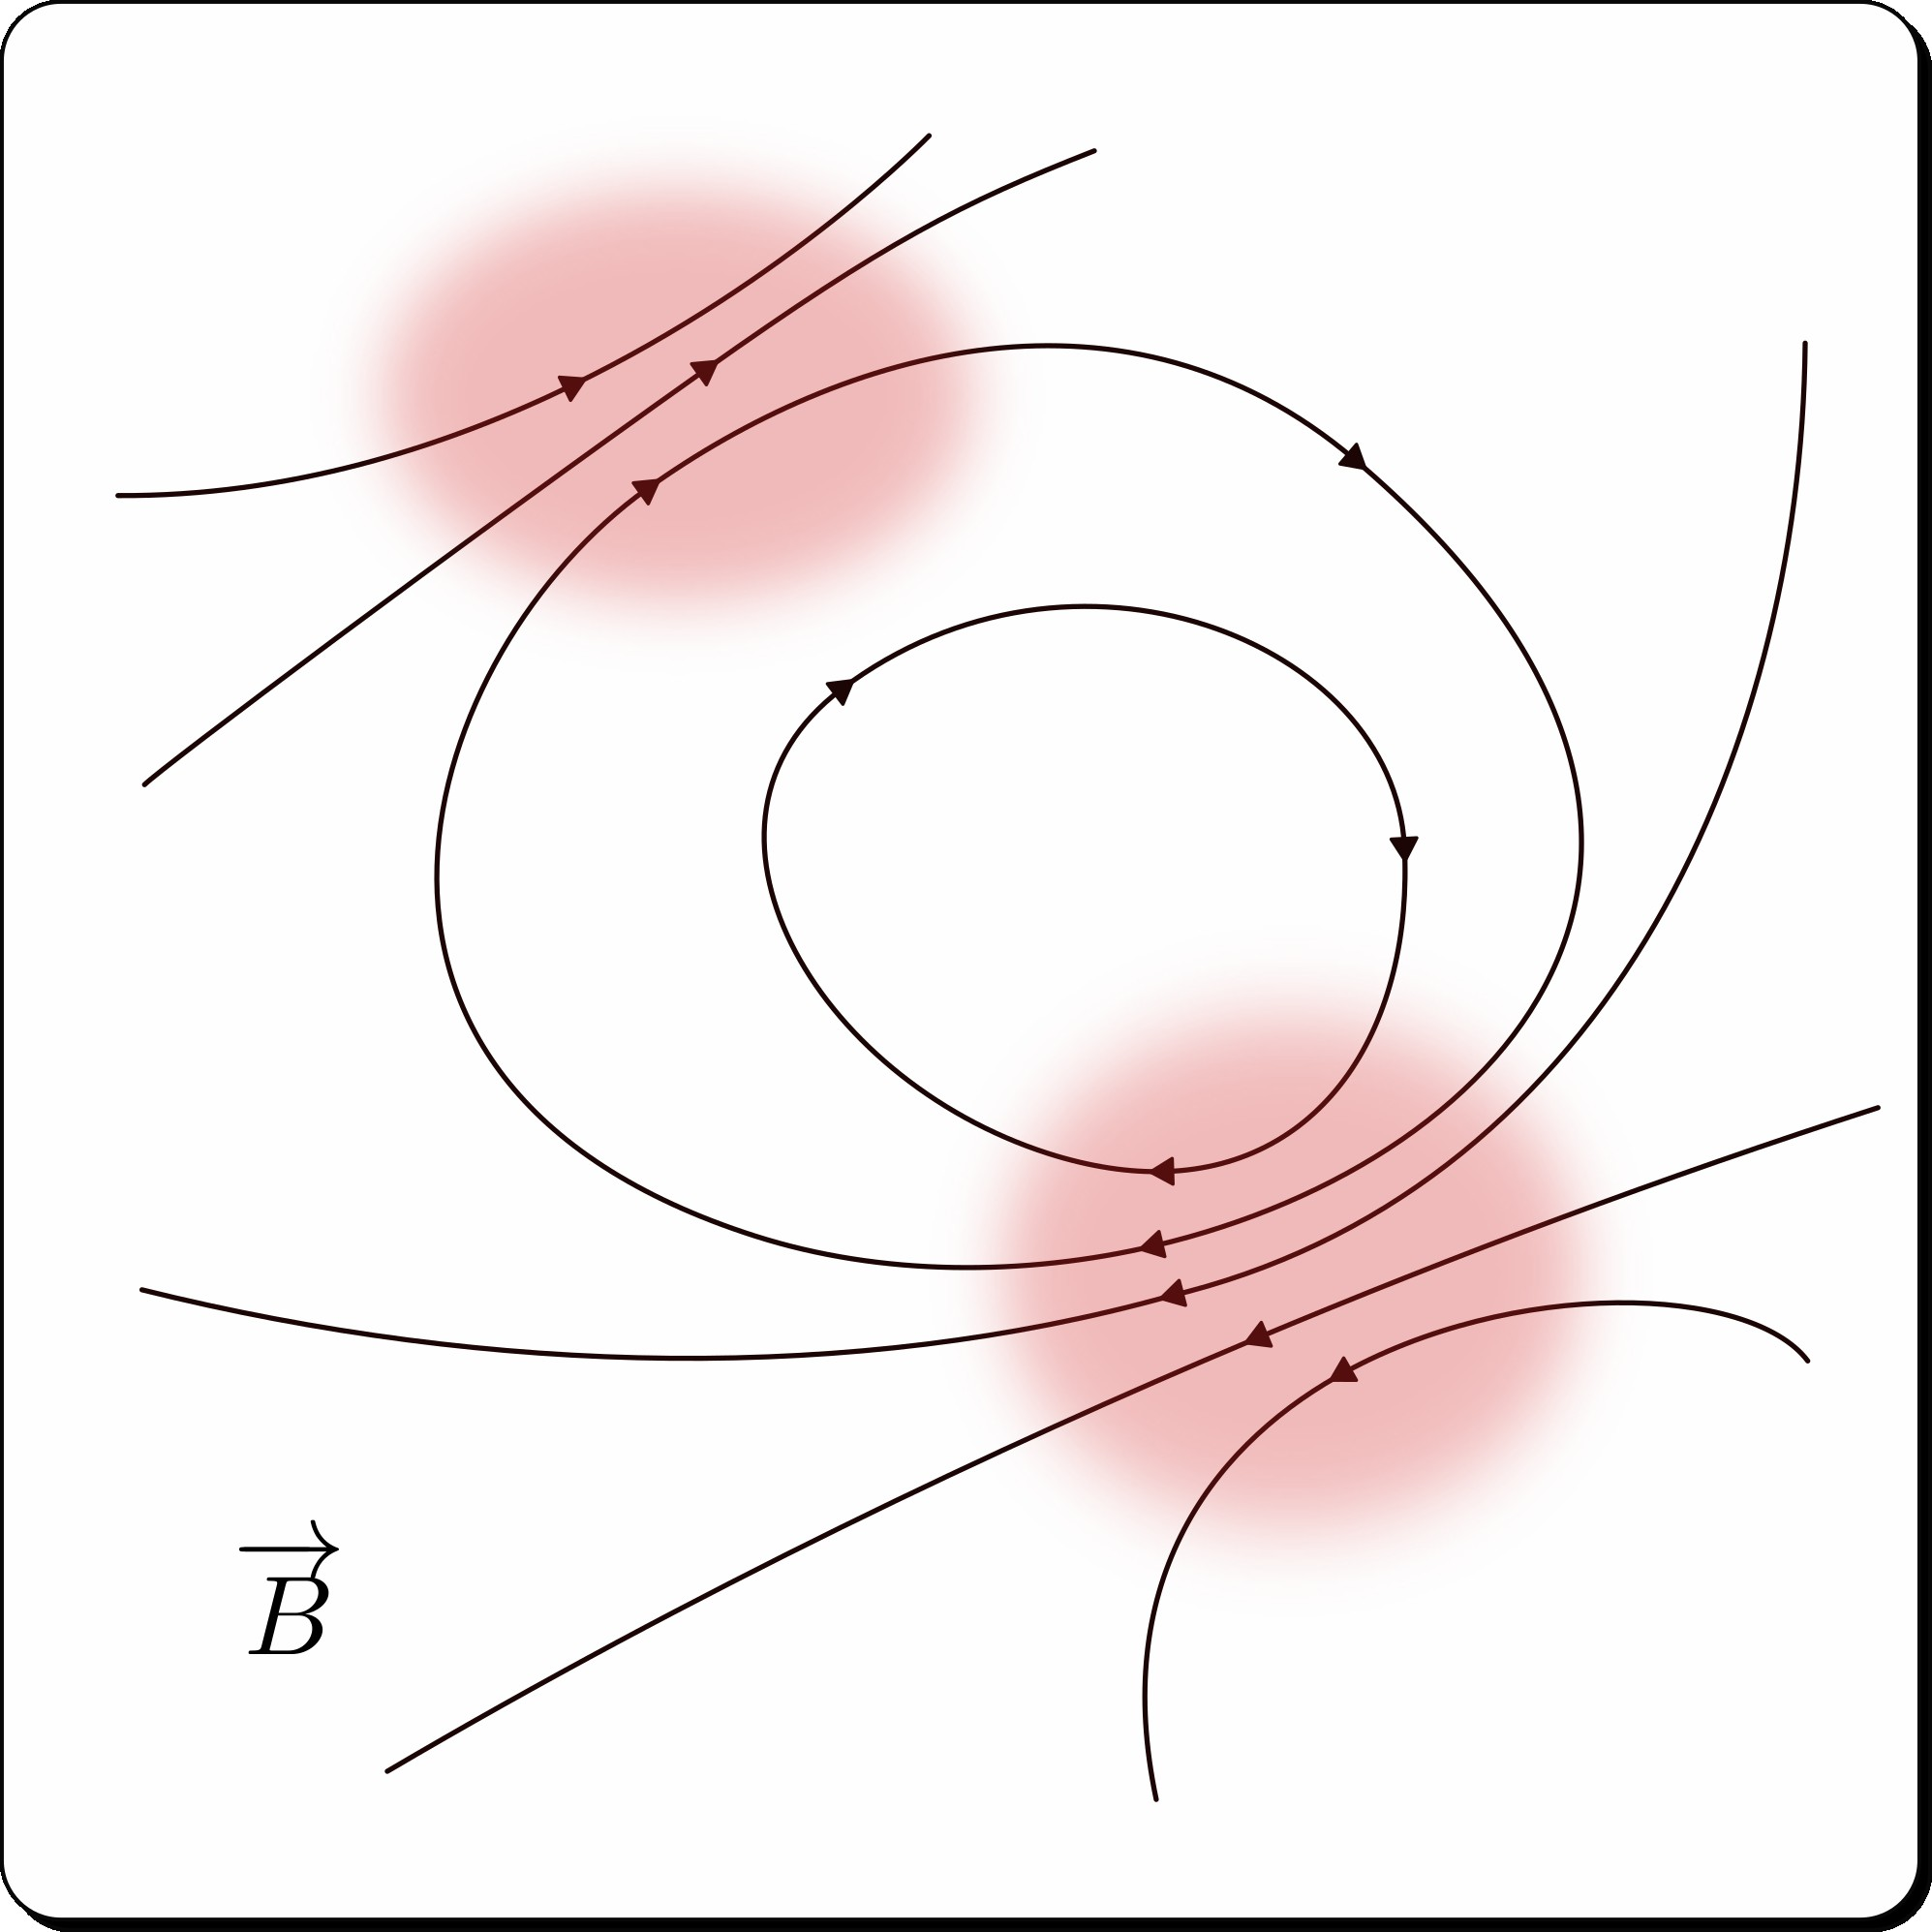
\includegraphics[width=\linewidth]{ldc_intens}
	\end{center}
\end{tcb*}

\subsection{Dispositifs créant un champ uniforme}
On a trois manière aisées de créer un champ uniforme~:
\begin{enumerate}
	\item \textbf{Dans un solénoïde}, les lignes de champ sont parallèles~;

	\item Entre les deux pôles d'un \textbf{aimant en U}, l'expérience avec la
	      limaille de fer montre que le champ est uniforme~;
	      \smallbreak
	      \begin{center}
		      \noindent
		      \begin{minipage}[c]{.45\linewidth}
			      \centering
			      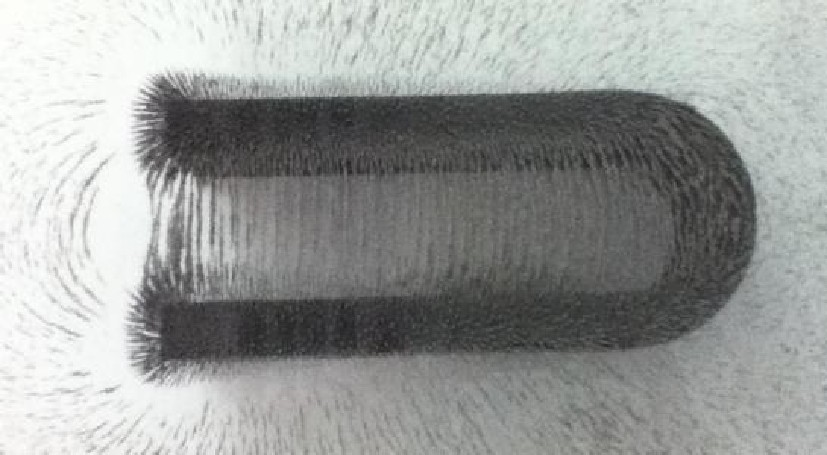
\includegraphics[scale=1,rotate=180]{aimu_lim.jpg}
			      % \captionof{figure}{Observation du champ magnétique dans un aimant en
			      %  U par limaille de fer.}
			      % \label{fig:aimu_lim}
		      \end{minipage}
		      \hfill
		      \begin{minipage}[c]{.45\linewidth}
			      \centering
			      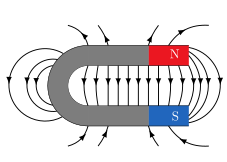
\includegraphics[scale=1]{aimu_sch}
			      % \captionof{figure}{Schématisation du champ magnétique dans un aimant en
			      %  U.}
			      % \label{fig:aimu_sch}
		      \end{minipage}
		      \captionof{figure}{Observation du champ créé par un aimant en U~:
			      limaille de fer et schématisation.}
		      \label{fig:aimu}
	      \end{center}

	\item
	      ~
	      \smallbreak
	      \vspace{-15pt}
	      \noindent
	      \begin{minipage}[c]{.60\linewidth}
		      On peut également créer un champ magnétique uniforme avec deux bobines
		      plates dans une configuration particulière~: deux \textbf{bobines de
			      rayon $R$} et \textbf{disposées à une distance $R$ l'une de l'autre}, si
		      elles sont parcourues par la même intensité, donnent un champ magnétique
		      uniforme entre elles. On appelle cet ensemble une \textbf{bobine de
			      \textsc{Helmoltz}}~; voir Figure~\ref{fig:helm}.
		      Vous pourrez pour cela manipuler une animation disponible en
		      ligne\footnote{\url{www.sciences.univ-nantes.fr/sites/genevieve_tulloue/Elec/Champs/Helmholtz_FJ.php}}.
	      \end{minipage}
	      \hfill
	      \begin{minipage}[c]{.38\linewidth}
		      \begin{center}
			      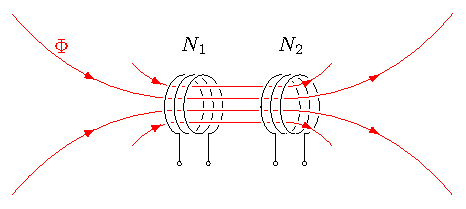
\includegraphics[width=\linewidth]{helmoltz}
			      \captionof{figure}{Bobine de \textsc{Helmoltz}, échelle non respectée.}
			      \label{fig:helm}
		      \end{center}

	      \end{minipage}
\end{enumerate}

% \begin{figure}[h]
% 	\centering
% 	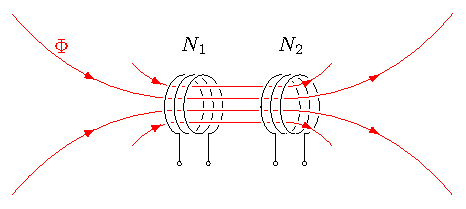
\includegraphics[width=.7\linewidth]{helmoltz}
%   \caption{Représentation des lignes de champ d'une bobine de \textsc{Helmoltz}.
%     Le schéma n'est pas exactement à l'échelle~: il faut que la distance entre
%   les bobines soit égale à leur rayon.}
% 	\label{fig:helm}
% \end{figure}

\subsection{Lien entre courant et champ magnétique}
\label{ssec:lienicour}
\subsubsection{Direction du champ magnétique}
\label{sssec:chpdir}
\begin{tcb*}(ror){Règles de la main droite}
	\begin{minipage}[t]{.45\linewidth}
		\begin{center}
			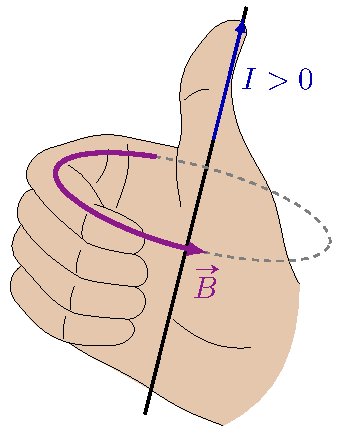
\includegraphics[width=.5\linewidth]{ra_fil}
			\label{fig:rafil}
			\captionof{figure}{Pour un champ créé par un fil~: pouce sur le courant,
				doigts selon $\protect\Bf$.}
		\end{center}
	\end{minipage}
	\hfill
	\begin{minipage}[t]{.45\linewidth}
		\begin{center}
			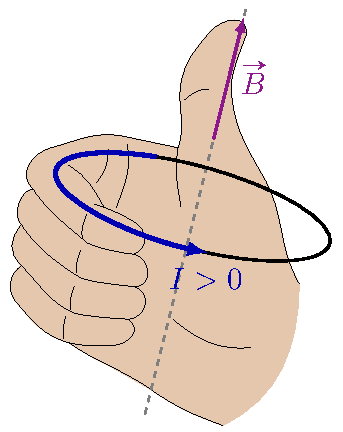
\includegraphics[width=.5\linewidth]{ra_bob}
			\label{fig:rabob}
			\captionof{figure}{Pour un champ créé par une bobine~: pouce sur
				$\protect\Bf$, doigts selon le courant.}
		\end{center}
	\end{minipage}
\end{tcb*}

\begin{tcb*}(inte){Analogie magnéto-mécanique}
	Pour se créer une intuition de la direction du champ créé par un aimant ou par
	une bobine, il est utile d'essayer de se représenter la bobine comme un
	\textbf{ventilateur sans pâle}, qui aspire lentement l'air en amont, puis
	rapidement en son milieu, pour l'éjecter ensuite de l'autre côté. L'aimant
	serait alors un tuyau d'aspirateur inversé.
\end{tcb*}

\begin{tcb}(appl)<lftt>'l'{Sens du courant et du champ}
	\centering
	\sswitch{
		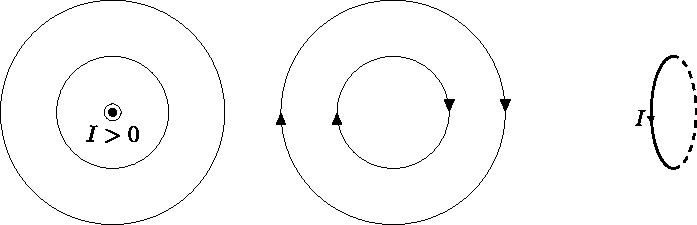
\includegraphics[scale=1]{ra_app-stud}
	}{
		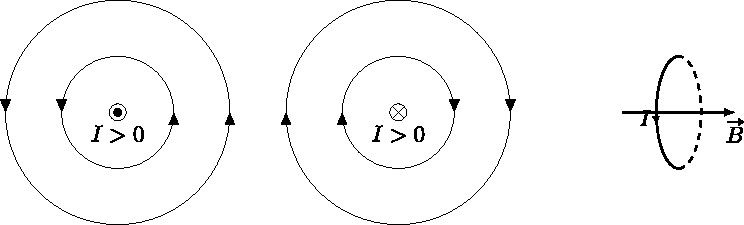
\includegraphics[scale=1]{ra_app}
	}
\end{tcb}

\subsubsection{Proportionnalité}
\label{sssec:prop}
\begin{tcb*}[sidebyside, righthand ratio=.35](prop){Relation courant-champ}
	\tcbsubtitle{\fatbox{\textbf{En général}}}
	Dans le vide, le champ magnétique créé par un courant $i$ est donné par~:
	\psw{%
		\[
			\boxed{\norm{\Bf} = \mu_0 \frac{i(t)}{L}}
		\]
	}%
	\vspace{-15pt}
	\begin{itemize}
		\item $i (t)$ le courant~;
		\item $\mu_0 = 4\pi\cdot \SI{e-7}{H.m ^{-1}}$ est la \textbf{perméabilité du
			      vide}~;
		\item $L$ est une longueur typique du système.
	\end{itemize}
	\tcblower
	\tcbsubtitle{\fatbox{\textbf{Solénoïde}}}
	À l'intérieur d'un solénoïde de $N$ spires où le champ est uniforme, on a
	\psw{%
		\[
			\boxed{\Bf = \mu_0ni (t)\uz}
		\]
	}%
	avec $\uz$ l'axe orienté selon la règle de la main droite par
	rapport au courant, et $n = \frac{N}{L}$ le nombre de spires par mètre.
\end{tcb*}

\subsubsection{Symétries de distribution et de champ}
\label{sssec:symdist}
Les situations qu'on a étudiées jusque-là ont toutes fait preuve d'une certaine
symétrie, et ce n'est pas un hasard.

\begin{tcb*}[list entry={\lte Plans d'(anti)-symétrie de distrib.}](defi){Plans d'(anti)-symétrie d'une distribution}
	Soit $\vv{j}(M)$ le vecteur de distribution de courant. Il peut
	posséder deux plans intéressants~:
	\smallbreak
	\begin{isd}[sidebyside align=top]
		\tcbsubtitle{\fatbox{\textbf{Plan de symétrie $\Pi\ind{s}$}}}
		Les courants en tous \textbf{points $P$ et $P'$ symétriques} par rapport à
		$\Pi\ind{s}$ sont \textbf{eux-mêmes symétriques}~:
		\[
			\small
			\vv{j}(P') = \sym_{\Pi\ind{s}} \vv{j}(P)
			\Lra
			\left\{
			\psw{%
				\begin{array}{rl}
					\vv{j}_{\parr}(P) & = +\vv{j}_{\parr}(P')
					\\[1em]
					\vv{j}_{\perp}(P) & = -\vv{j}_{\perp}(P')
				\end{array}
			}%
			\right.
		\]
		\begin{center}
			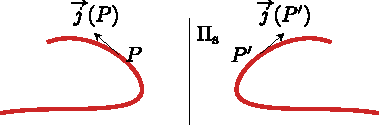
\includegraphics[height=2.5cm]{Psym_j}
		\end{center}
		\tcblower
		\tcbsubtitle{\fatbox{\textbf{Plan d'antisymétrie $\Pi\ind{a}$}}}
		Les courants en tous \textbf{points $P$ et $P'$ symétriques} par rapport à
		$\Pi\ind{s}$ sont \textbf{antisymétriques}~:
		\[
			\small
			\vv{j}(P') = -\sym_{\Pi\ind{a}} \vv{j}(P)
			\Lra
			\left\{
			\psw{%
				\begin{array}{rl}
					\vv{j}_{\parr}(P) & = -\vv{j}_{\parr}(P')
					\\[1em]
					\vv{j}_{\perp}(P) & = +\vv{j}_{\perp}(P')
				\end{array}
			}%
			\right.
		\]
		\begin{center}
			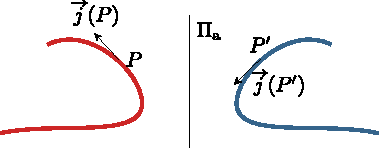
\includegraphics[height=2.5cm]{Pasym_j}
		\end{center}
	\end{isd}
\end{tcb*}

L'étude des symétries est toute une science en soit, qui a mené à une des plus
grandes découvertes scientifiques du monde~: le théorème de
\textsc{Noether}\footnote{Figure incontournable de la physique moderne, Emmy
	\textsc{Noether} était une mathématicienne hors pair, reconnue dans le monde
	scientifique à une époque où les femmes étaient encore plus minimisées
	qu'aujourd'hui. \textsc{Einstein} aurait qualifié son théorème de «~monument
	de la pensée mathématique~».}, démontré en 1915.

Dans le cas du champ magnétique, on obtient les résultats suivants~:

\begin{tcb*}(ror){Symétries}
	Soit M un point, $\Pi\ind{s}$ un plan de symétrie de la distribution, et
	$\Pi\ind{a}$ un plan d'\textbf{anti}symétrie. Pour le champ $\Bf$, on
	obtient~:
	\smallbreak
	\begin{isd}[sidebyside align=top]
		\tcbsubtitle{\fatbox{\textbf{Plan de symétrie $\Pi\ind{s}$}}}
		Pour $M$ et $M'$ symétriques par rapport à $\Pi\ind{s}$, le champ $\Bf$ est
		\textbf{anti-symétrique} par rapport à $\Pi\ind{s}$~:
		\begin{gather*}
			\Bf(M') = -\sym_{\Pi\ind{s}} \left(\Bf(M)\right)
			\\\Lra
			\left\{
			\psw{%
				\begin{array}{rl}
					\Bf_{\parr}(M) & = -\Bf_{\parr}(M')
					\\[1em]
					\Bf_{\perp}(M) & = +\Bf_{\perp}(M')
				\end{array}
			}%
			\right.
		\end{gather*}
		\begin{center}
			\sswitch{
				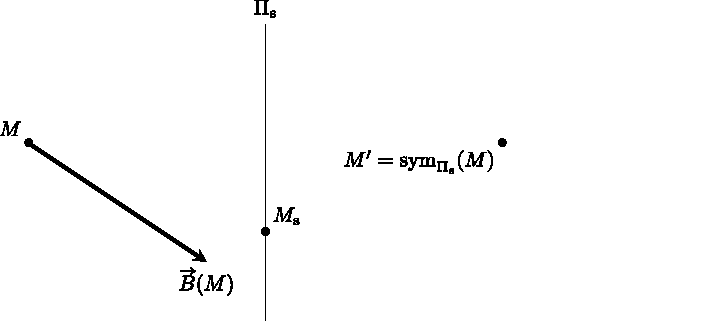
\includegraphics[width=\linewidth]{Psym_B-stud}
			}{
				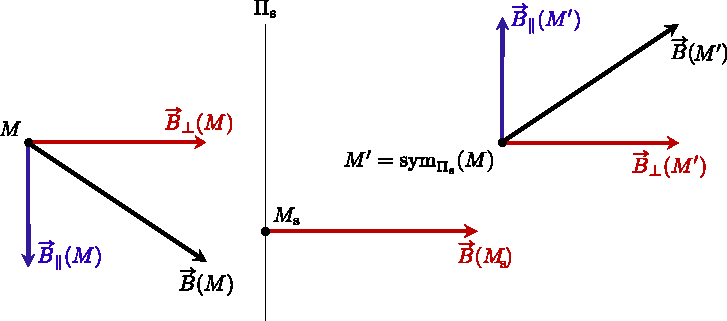
\includegraphics[width=\linewidth]{Psym_B}
			}
		\end{center}
		On retiendra
		\[
			\setlength{\fboxsep}{3mm}
			\forall M\ind{s} \in \Pi\ind{s},
			\boxed{
				\psw{%
					\Bf (M\ind{s}) \perp \Pi\ind{s}
				}%
			}
		\]
		\tcblower
		\tcbsubtitle{\fatbox{\textbf{Plan d'antisymétrie $\Pi\ind{a}$}}}
		Pour $M$ et $M'$ symétriques par rapport à $\Pi\ind{a}$, le champ $\Bf$ est
		\textbf{symétrique} par rapport à $\Pi\ind{a}$~:
		\begin{gather*}
			\Bf(M') = \sym_{\Pi\ind{a}} \left(\Bf(M)\right)
			\\\Lra
			\left\{
			\psw{%
				\begin{array}{rl}
					\Bf_{\parr}(M) & = +\Bf_{\parr}(M')
					\\[1em]
					\Bf_{\perp}(M) & = -\Bf_{\perp}(M')
				\end{array}
			}%
			\right.
		\end{gather*}
		\begin{center}
			\sswitch{
				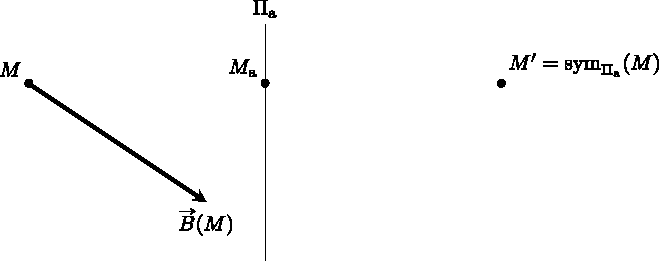
\includegraphics[width=\linewidth]{Pasym_B-stud}
			}{
				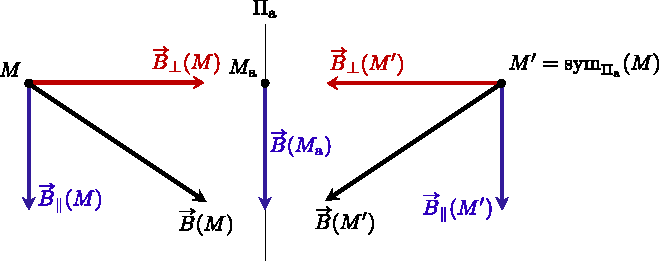
\includegraphics[width=\linewidth]{Pasym_B}
			}
		\end{center}
		On retiendra
		\[
			\setlength{\fboxsep}{3mm}
			\forall M\ind{a} \in \Pi\ind{a},
			\boxed{
				\psw{%
					\Bf (M\ind{a}) \in \Pi\ind{a}
				}%
			}
		\]
	\end{isd}
	% \psw{
	% 	\begin{itemize}
	% 		\item $\Mr \in \Pi\ind{s} \Lra \vv{B}(M) \perp \Pi\ind{s}$~;
	% 		\item $\Mr \in \Pi\ind{a} \Lra \vv{B}(M) \in \Pi\ind{a}$.
	% 	\end{itemize}
	% }
\end{tcb*}
\begin{tcb}[breakable, sidebyside](appl)<lftt>{Symétrie distribution/champ}
	\begin{enumerate}
		\item Soit un fil doté de coordonnées cylindriques. Étudions ses symétries~:
		      \begin{center}
			      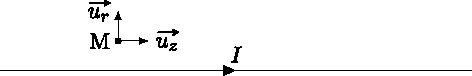
\includegraphics[scale=1]{sym1}
		      \end{center}
		      \vspace{-15pt}
		      \psw{
			      \begin{itemize}
				      \item $\Pi\ind{a} = (\Mr,\ur,\ut)$ est plan de
				            d'\textbf{anti}symétrie de la distribution (si on fait le miroir
				            du courant il va dans le sens opposé), donc $\vv{B} \in
					            \Pi\ind{a}$.
				      \item $\Pi\ind{s} = (\Mr,\ur,\uz)$ est plan de \textbf{symétrie}
				            de la distribution~:
				            $\vv{B} \perp \Pi\ind{s} \Ra \vv{B} \parr \ut$.
			      \end{itemize}
		      }
	\end{enumerate}
	\tcblower
	\begin{enumerate}[start=2]
		\item Soit un solénoïde avec des coordonnées cylindriques.
		      \begin{center}
			      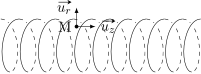
\includegraphics[scale=1]{sym2}
		      \end{center}
		      \vspace{-15pt}
		      \psw{
			      \begin{itemize}
				      \item $\Pi\ind{s} = (\Mr,\ur,\ut)$ plan de \textbf{symétrie}~:
				            $\vv{B} \perp \Pi\ind{s} \Ra \vv{B} \parr \uz$.
			      \end{itemize}
		      }
	\end{enumerate}
\end{tcb}
\subsubsection{Invariances de la distribution de courants}
\label{sssec:invdist}
\begin{tcb*}(ror){Invariances}
	\begin{center}
		\psw{
			Le champ $\vv{B}$ possède les mêmes \textbf{invariances} que la
			distribution de courant
		}
	\end{center}
\end{tcb*}

\begin{tcb*}[sidebyside, sidebyside align=top](impo){Différence invariance/symétrie}
	\tcbsubtitle{\fatbox{\textbf{Symétrie}}}
	\textbf{Spécifique} à chaque champ, dépend d'un \textbf{plan miroir} de la
	distribution, donne la \textbf{direction}.
	\tcblower
	\tcbsubtitle{\fatbox{\textbf{Invariance}}}
	\textbf{Général}, dépend d'une \textbf{translation} ou \textbf{rotation} de
	la distribution, donne la dépendence aux \textbf{coordonnées}.
\end{tcb*}

\begin{tcb}(appl)<lftt>'l'{Invariances distribution/champ du fil infini}
	Étudions les invariances de la distribution dans le cas du fil infini~:
	\begin{enumerate}
		\item
		      \psw{%
			      Pour un fil infini par exemple, le translater selon $z$ ne change pas
			      la distribution. Il n'y a donc aucune raison que $\vv{B}$ dépende de
			      $z$.
		      }%
		\item
		      \psw{%
			      De la même manière, pour tout fil parcouru par un courant, on a
			      invariance de la distribution par rotation selon $\theta$~: $\vv{B}$ ne
			      saurait dépendre de $\theta$.
		      }%
	\end{enumerate}
	Autrement dit, par l'étude des invariances pour un fil infini, on
	sait que
	\psw{%
		\[
			\vv{B}(r,\dcancel{\theta},\dcancel{z})
		\]
	}%
	Si on ajoute l'étude des symétries, on a que $\vv{B}\parr \ut$. Tout combiné,
	on a donc
	\psw{%
		\[
			\boxed{\vv{B}(\Mr) = B(r)\ut}
		\]
	}%
	\vspace{-30pt}
\end{tcb}

\begin{tcb*}[breakable](appl){Exercice bilan sur lignes de champ}
	Les cartes de champ magnétique ci-dessous sont des vues en coupe du champ
	produit par des spires de courant circulaires. Dans les deux cas, indiquer
	\begin{tasks}[label=\protect\fbox{\arabic*}](2)
		\task la position des sources
		\task le sens du courant circulant dans les spires
		\task les zones de champ fort et faible
		\task le cas échéant s'il existe une zone de l'espace où le champ magnétique
		est uniforme.
	\end{tasks}
	\begin{center}
		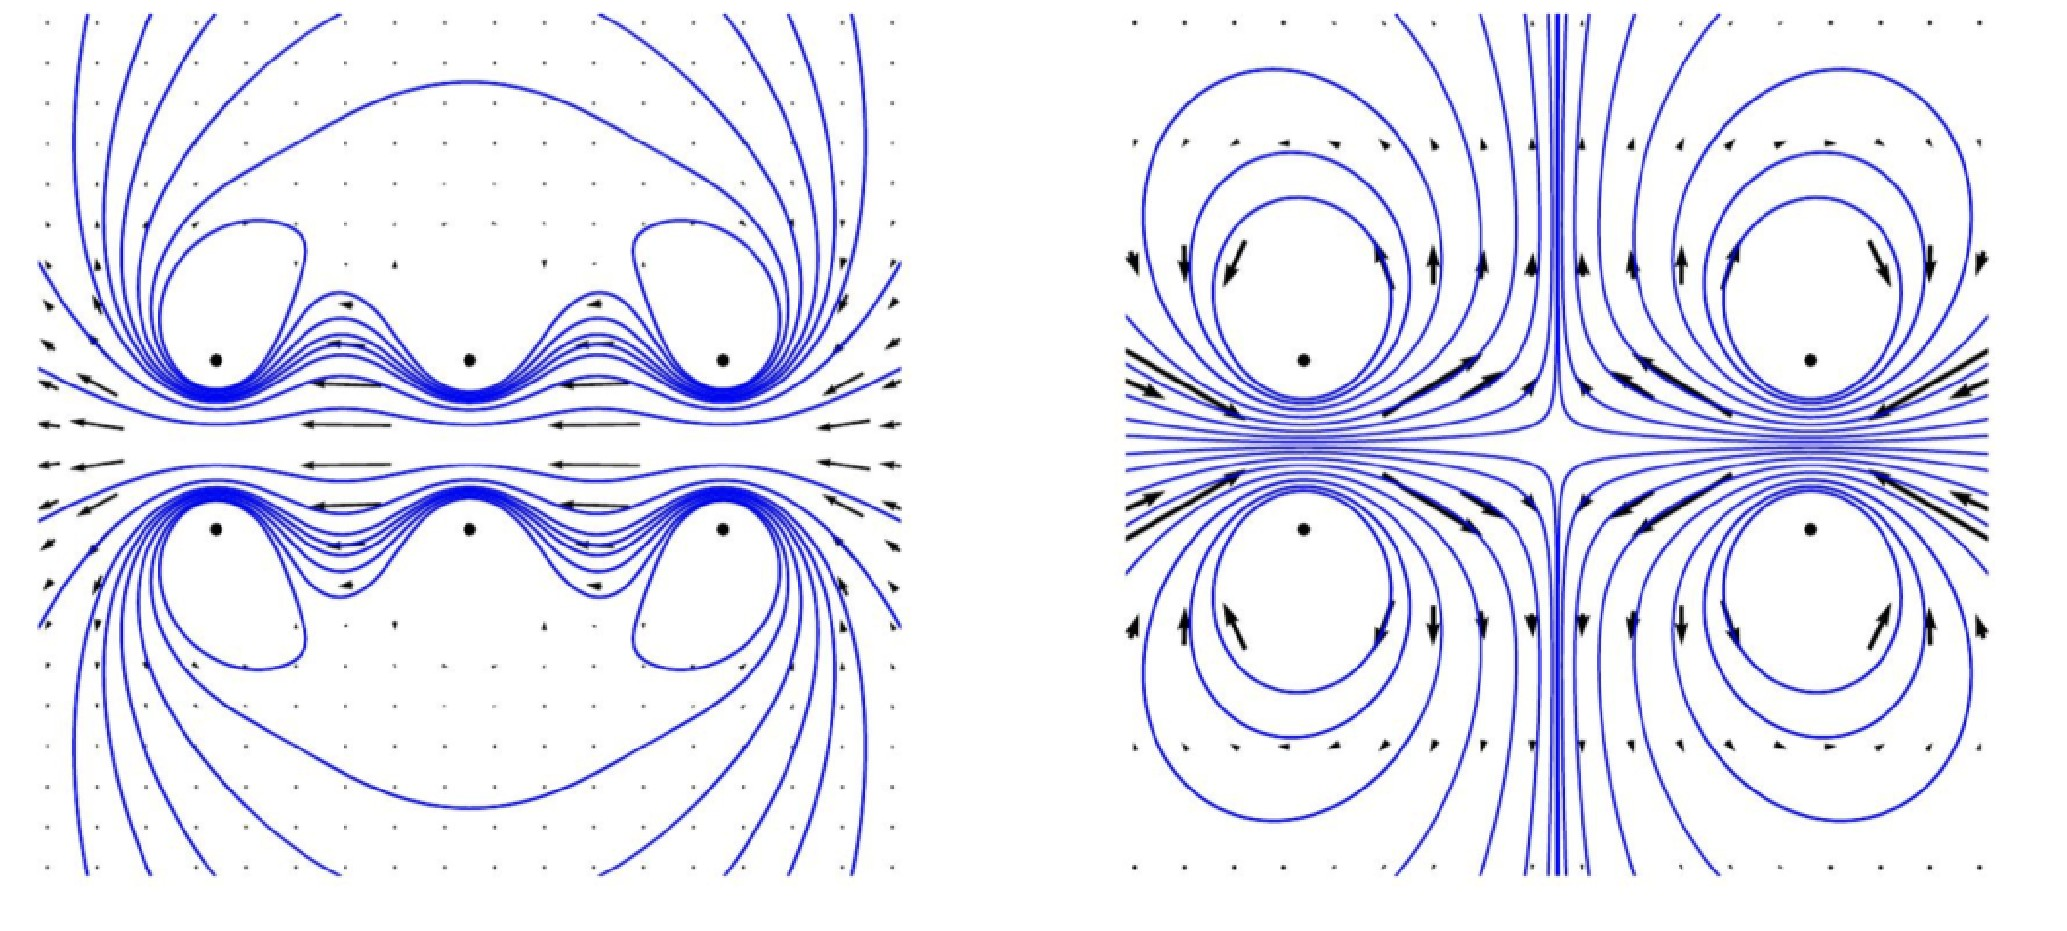
\includegraphics[scale=.8]{ldc_bilan.jpg}
		% \captionof{figure}{Représentation des lignes de champ pour différentes
		% situations avec des pires de courant.}
	\end{center}
\end{tcb*}

\vspace*{-10pt}

\section{Le moment magnétique}
\label{sec:momag}
\begin{tcb*}[sidebyside, righthand ratio=.2](defi){Moment magnétique}
	On remarque que les champs magnétiques créés par un aimant droit et par une
	spire se ressemblent. On les modélise donc par le \textbf{même objet
		mathématique} appelé \textbf{moment magnétique} $\muf$ ou $\mf$, caractérisé
	par le \textbf{champ qu'il produit}.
	\tcblower
	\begin{center}
		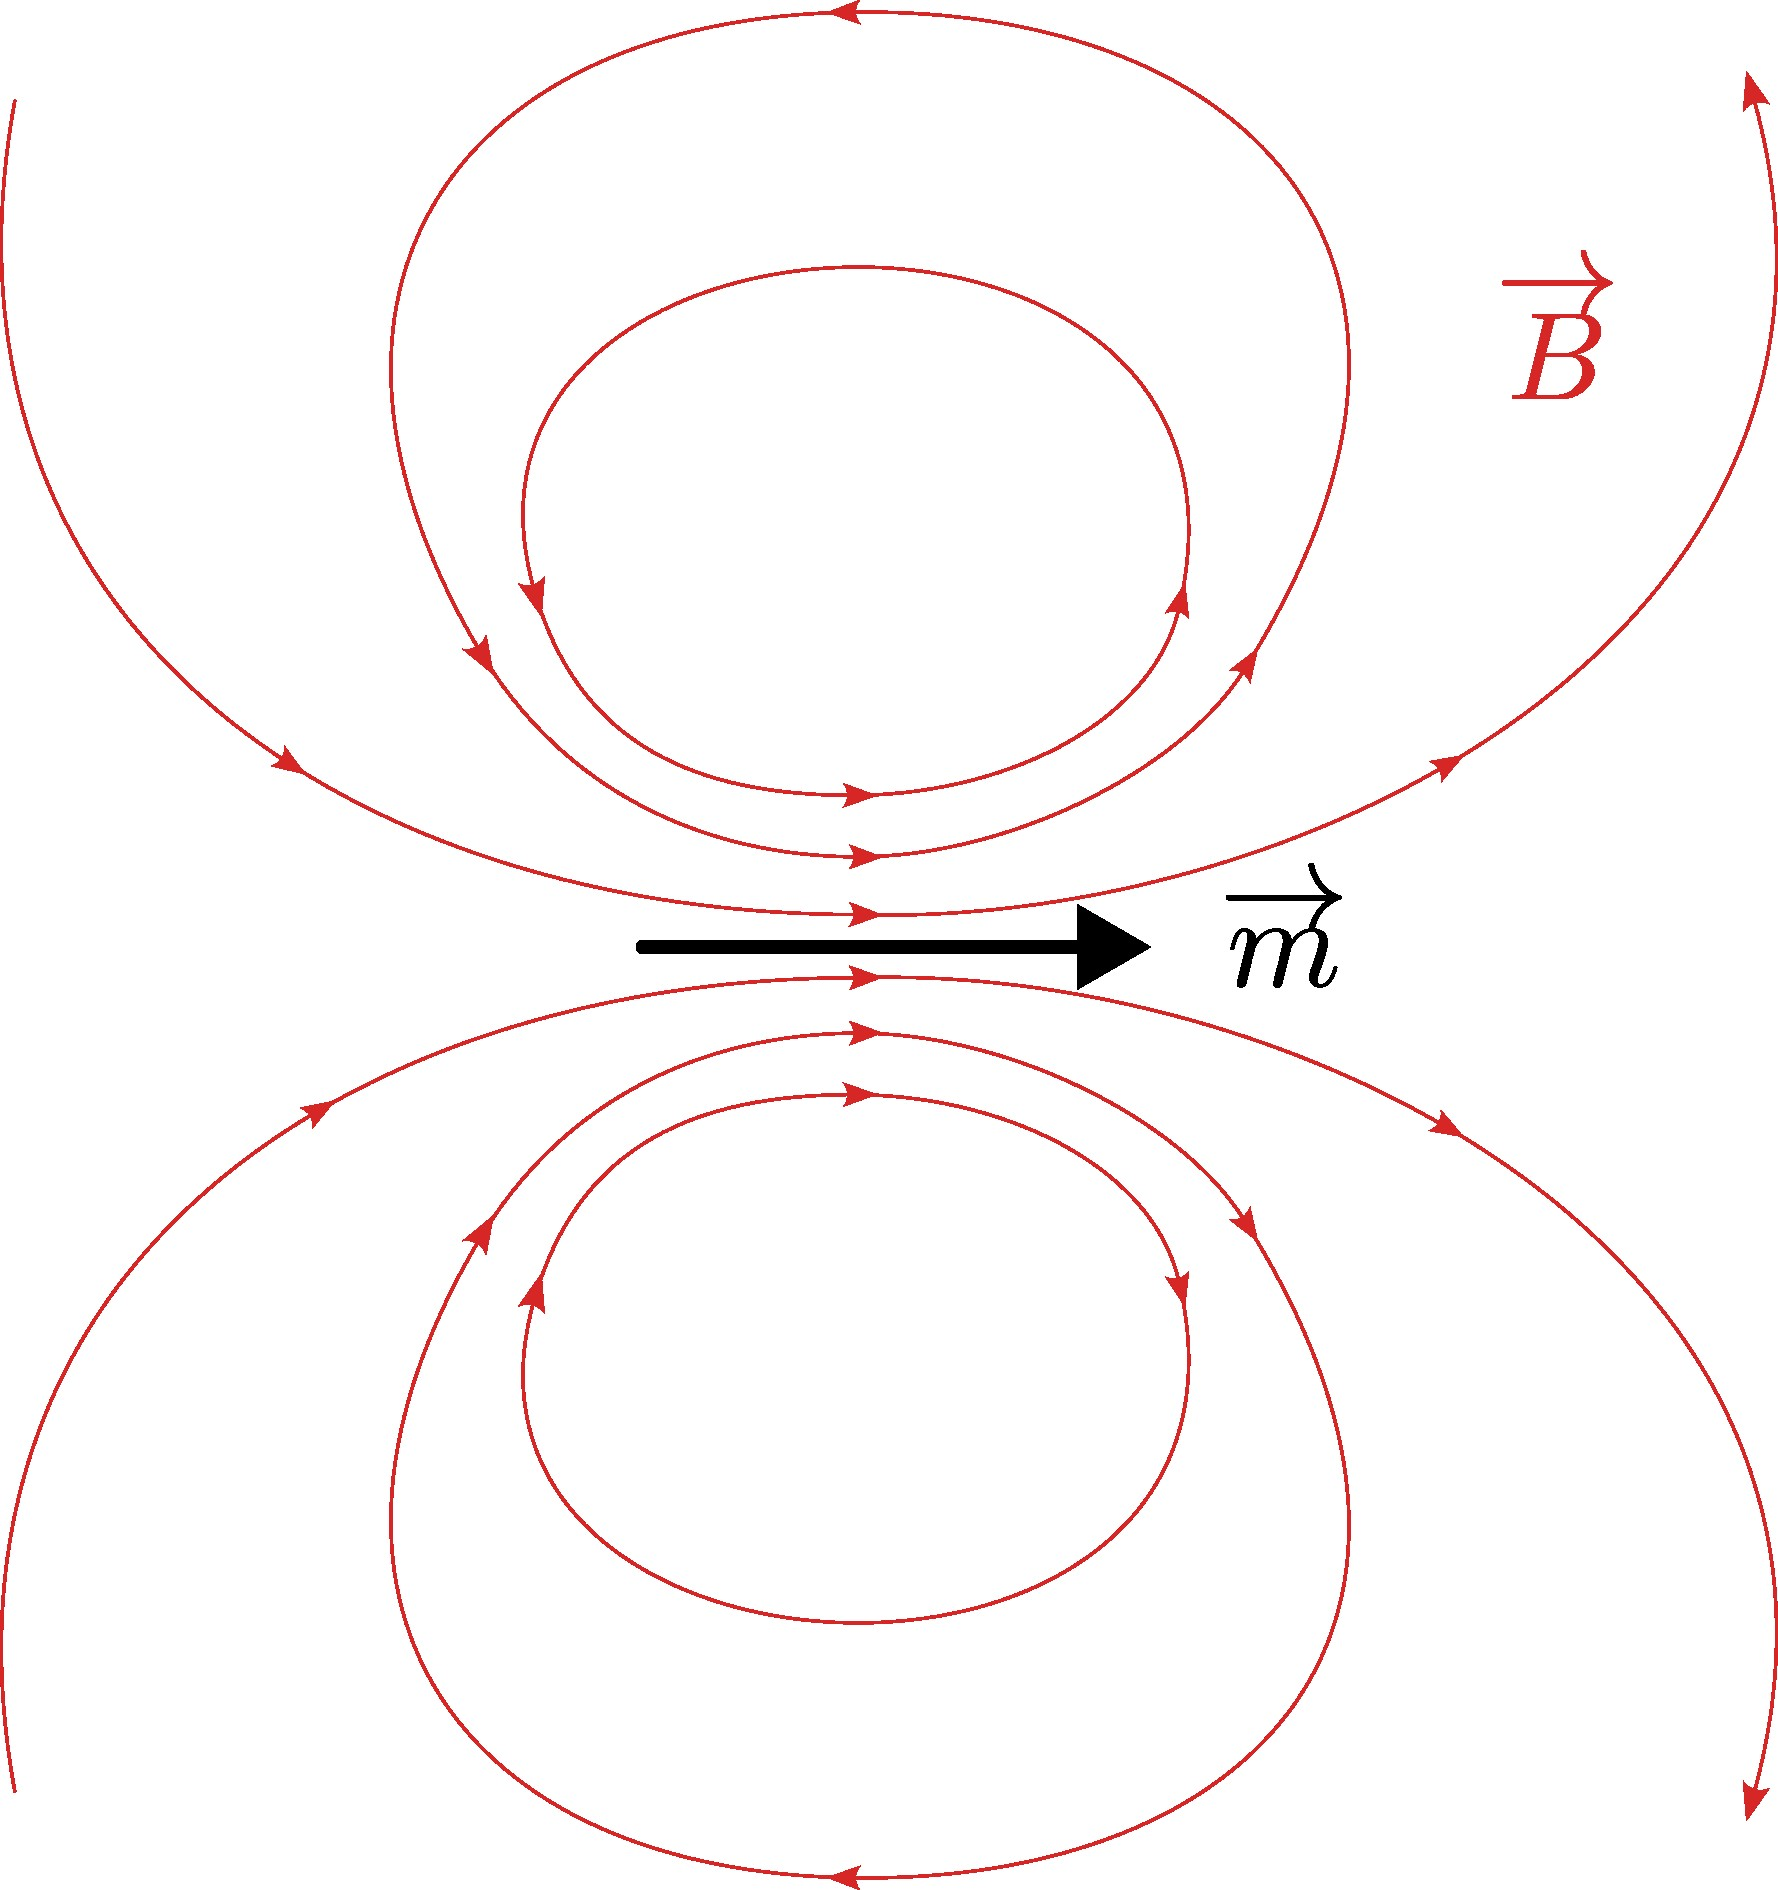
\includegraphics[width=\linewidth]{momag_gen}
	\end{center}
\end{tcb*}

\subsection{Boucle de courant}
\label{ssec:magboucle}
\begin{tcb*}[sidebyside, righthand ratio=.2](prop){Moment magnétique d'une spire}
	On considère une spire de rayon $R$ parcourue par un courant $i$. La normale à
	la surface est notée $\vv{n}$, orientée dans le sens de la main droite par
	rapport au courant.
	\smallbreak
	Le \textbf{moment magnétique} $\vv{\mu}$ de la spire plane est
	\[
		\psw{\boxed{\vv{\mu} = i \vv{S} = i\pi R^2 \vv{n}}}
		\qMath{en}
		\psw{\boxed{\si{A.m^2}}}
	\]
	\tcblower
	\begin{center}
		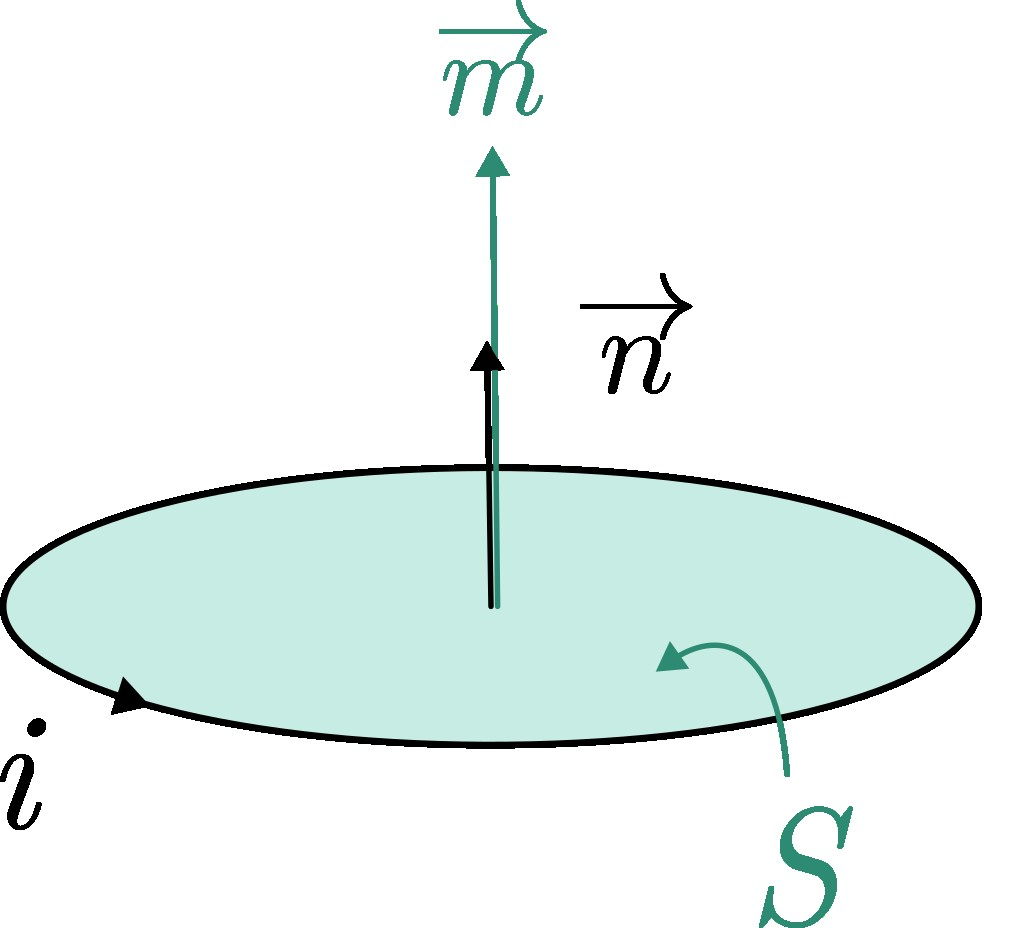
\includegraphics[width=\linewidth]{momag_spire}
	\end{center}
\end{tcb*}

Dans ce cas, c'est le mouvement de \textbf{particules chargées} qui créé le
champ magnétique. Cette notion s'applique également aux bobines.

\subsection{Cas des aimants}
\label{ssec:magaim}
\begin{wrapfigure}[2]{r}{0.2\textwidth}
	\vspace*{-35pt}
	\begin{center}
		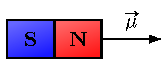
\includegraphics[scale=1]{momag_aimdroit}
	\end{center}
\end{wrapfigure}
La notion de moment magnétique s'applique aussi aux aimants, même si sa source
n'est pas due à un mouvement de translation comme peut l'être le courant dans un
fil~: la source du magnétisme dans les aimants est intrinsèquement
\textbf{quantique}, et vient de la nature «~aimantée~» des électrons. On
distingue deux sources~:
\begin{itemize}
	\item[b]{Moment magnétique orbital} dû au mouvement des électrons autour d'un
	noyau atomique, dessinant une boucle de courant auquel on associe un moment
	magnétique~;
	\item[b]{Moment magnétique de spin} propriété intrinsèque des particules
	élémentaires. Elle n'a \textbf{pas d'équivalent classique}.
\end{itemize}
Ce sont ensuite des effets à grande échelle qui permettent l'existence d'un
champ à l'échelle d'un solide entier, selon l'orientation moyenne des moments
microscopiques\ftn{Pour plus de détails, voir
	\url{https://www.youtube.com/watch?v=hFAOXdXZ5TM}.}.

\begin{center}
	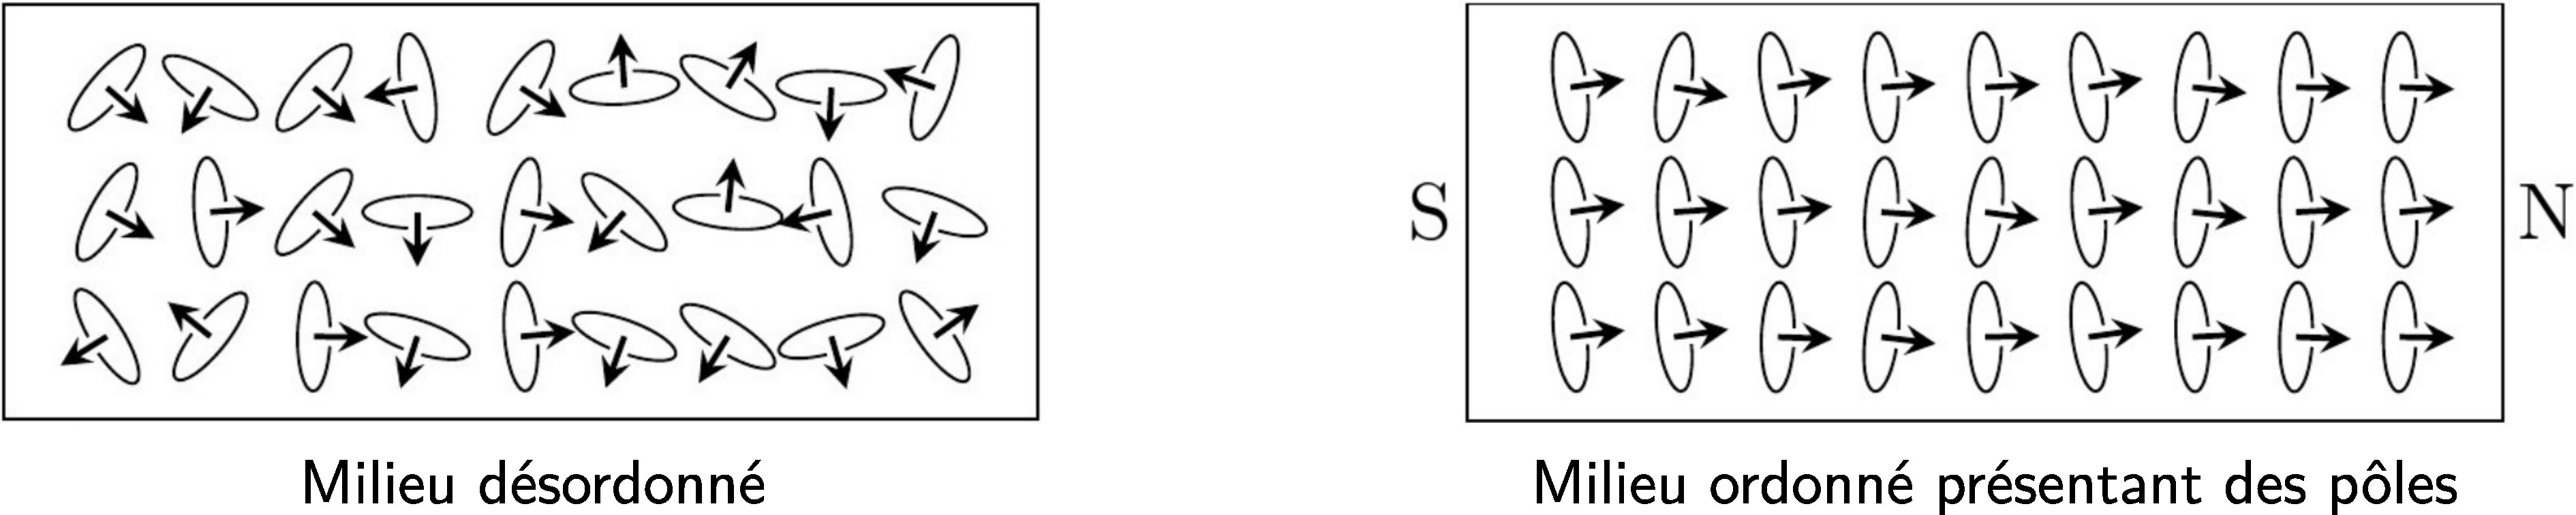
\includegraphics[scale=.8]{momag_aimdroit-qtq}
\end{center}

\begin{tcb*}(odgr)<lftt>'l'{Moment magnétique d'un aimant}
	On a comme ordre de grandeur~: aimant droit $\approx \SI{1}{A.m^2}$~; aimant
	néodyme $\approx \SI{10}{A.m^2}$~; pour la Terre $\approx \SI{8e22}{A.m^2}$.
\end{tcb*}
\vspace{-15pt}
\end{document}
